\documentclass[a4paper, 10pt]{article}

\usepackage{tabularx} % extra features for tabular environment
\usepackage{amsmath}  % improve math presentation
\usepackage{graphicx} % takes care of graphic including machinery
\usepackage[margin=1in,letterpaper]{geometry} % decreases margins
\usepackage{cite} % takes care of citations
\usepackage[final]{hyperref} % adds hyper links inside the generated pdf file
\usepackage{ctex}
\usepackage{titlesec}
%\usepackage{CJKutf8, CJK}
\usepackage{makecell}                 % 三线表-竖线
\usepackage{booktabs}                 % 三线表-短细横线
% \usepackage{natbib}
\usepackage{graphicx}				  % 表格单元格逆时针
\usepackage{multirow}				  % 合并单元格
\usepackage{array}
\usepackage{amssymb}				  % 勾
\usepackage{amsmath}
\usepackage{longtable}                % 导入 longtable 宏包,表格自动换行
\usepackage{caption}
\usepackage{subcaption}               % 设置子图
\usepackage{color}					  % 文本颜色包
\usepackage{xcolor}
\usepackage{bbm}					  % 输入指示函数
\usepackage{tablefootnote}			  % 表格注释
\usepackage{pythonhighlight}
\usepackage{fancyhdr}
\usepackage{lastpage}
\usepackage{tocloft}
\pagestyle{fancy}
\fancyhf{}
\fancyhead{}
\fancyfoot{}
\fancyhead[R]{\small Page \thepage\ of \pageref*{LastPage}}
\fancyhead[L]{\small Report}

\usepackage{listings}                 % 导入代码块
\usepackage{xcolor}
\lstset{
	numbers=left, 
	tabsize=1,
	columns=flexible, 
	numberstyle=  \small, 
	keywordstyle= \color{ blue!70},
	commentstyle= \color{red!50!green!50!blue!50}, 
	frame=shadowbox, % 阴影效果
	rulesepcolor= \color{ red!20!green!20!blue!20} ,
	escapeinside=``, % 英文分号中可写入中文
	xleftmargin=2em,
	xrightmargin=2em, 
	aboveskip=1em,
} 

\hypersetup{
	colorlinks=true,       % false: boxed links; true: colored links
	linkcolor=blue,        % color of internal links
	citecolor=blue,        % color of links to bibliography
	filecolor=magenta,     % color of file links
	urlcolor=blue         
}
%++++++++++++++++++++++++++++++++++++++++
\titleformat{\section}{\Large\bfseries\songti}{\thesection}{1em}{}
\titleformat{\subsection}{\large\bfseries\songti}{\thesubsection}{1em}{}
\titleformat{\subsubsection}{\normalsize\bfseries\songti}{\thesubsubsection}{1em}{}
\titleformat{\paragraph}{\small\bfseries\songti}{\paragraph}{1em}{}
\titleformat{\subparagraph}{\footnotesize\bfseries\songti}{\subparagraph}{1em}{}

\begin{document}
	
	
	\title{\songti \zihao{4}10-11月工作汇报}
	\author{\textrm{Ku Jui}}
	\date{\textrm{Oct - Nov 2023}}
	\maketitle
	
	\renewcommand{\figurename}{Figure} % 可以重新定义abstract,因为ctex会覆盖thebibliography
	% 	\begin{abstract}
		%		In this experiment we studied a very important physical effect by measuring the
		%		dependence of a quantity $V$ of the quantity $X$ for two different sample
		%		temperatures.  Our experimental measurements confirmed the quadratic dependence
		%		$V = kX^2$ predicted by Someone's first law. The value of the mystery parameter
		%		$k = 15.4\pm 0.5$~s was extracted from the fit. This value is
		%		not consistent with the theoretically predicted $k_{theory}=17.34$~s. We attribute %this
		%		discrepancy to low efficiency of our $V$-detector.
		%	\end{abstract}
	
	\renewcommand{\tablename}{Table}
	
	% 设置目录标题为居中
	\renewcommand{\cfttoctitlefont}{\hfill\Large\bfseries\songti}
	\renewcommand{\cftaftertoctitle}{\hfill}
	\renewcommand{\contentsname}{Content}
		
	\tableofcontents
	
	
	\part{Pre-Knowledge}	
	
	\section{方向}
		
%		弱光图像增强是图像处理领域的一个关键任务,旨在提升低光环境下拍摄图像的视觉质量。该领域的最新进展主要由深度学习技术推动,涵盖了多种学习策略、网络架构、损失函数和训练数据集的应用。低光图像增强在视觉监控、自动驾驶和计算摄影等多个领域均有广泛应用。特别是在智能手机摄影领域,由于相机光圈大小、实时处理需求和存储限制,低光环境下的图像拍摄面临着显著挑战。
%		
%		传统的低光增强方法,如基于直方图均衡和Retinex模型的方法,尽管在某些情况下有效,但也存在明显局限。例如,Retinex模型通常忽略噪声问题,可能导致增强结果中噪声的保留或放大;有效的先验或正则化的选择具有挑战性,不准确的先验可能导致伪影和颜色偏差;此外,这些方法的复杂优化过程也导致了较长的运行时间。
%		
%		近年来,基于深度学习的低光图像增强(LLIE)方法取得了显著的成功。与传统方法相比,基于深度学习的解决方案在准确性、鲁棒性和速度方面表现更佳,因此受到了越来越多的关注。然而,现有研究主要集中在亮度细化上,而忽视了色度的重要性。此外,这些方法在优化弱光图像与真实图像之间的外观距离时,往往忽略了物体边缘的模糊问题,这可能导致图像细节的损失,从而影响最终的结构相似性指数(SSIM)。
%		
%		针对极暗或极亮区域中图像边缘细节恢复的问题,一些研究者提出了在暗区域中加入敏感边缘先验的方法,以降低优化过程中的不适定性,并采用基于编码器-解码器的网络结构和回归损失来执行结构建模。进一步的研究提出了改进的模型,以解决弱光图像中局部边缘失真的问题,并对边缘图与弱恢复图的融合策略进行了优化。
%		
%		本研究提出了三个主要的创新点:首先,提出了一种基于CNN-Transformer并行架构的低光图像增强方法,用于有效地增强低光图像;其次,开发了一种从低光图像中直接提取边缘结构的多曝光策略;最后,提出了一种并联方法,用于融合边缘图和初步恢复的图像。
		
		根据目前的文献研究,在 LLIE 任务中,一种方法是采用边缘检测思想来引导弱光图像增强\footnote{为什么要采用图像的边缘图片来指导弱光图像恢复?
		首先,图像边缘图仅需要很少的数据量,其剔除了不相关的信息,保留了图像重要的结构属性。其次,低光图像通常具有很高的对比度,现有的方法可能无法在极暗或极亮的区域恢复图像边缘细节。同时,当物体边缘不清晰时,像素级损失往往会模糊边缘,破坏图像细节。而加入边缘先验可以降低优化外观重构时的不适定程度。最后,人类视觉系统对边缘高度敏感,保留结构信息对图像重建任务的性能至关重要。定义边缘可以通过学习区分黑暗区域的不同物体来指导增强过程,而不仅仅是识别低光区域。通过保留图像中的结构属性,这使得物体之间的可见性更好。},其策略是将边缘图与\textbf{初步恢复的图像}进行串联,然后通过单一的增强网络来实现最终的图像恢复(见Fig. \ref{fig: EEMEFN})。恢复结果的质量往往会受到最后的增强网络设计和初步恢复图像所包含特征与真实图像特征之间的相似度的影响。
		
		\begin{figure}[htbp]
			% read manual to see what [ht] means and for other possible options
			\centering 
			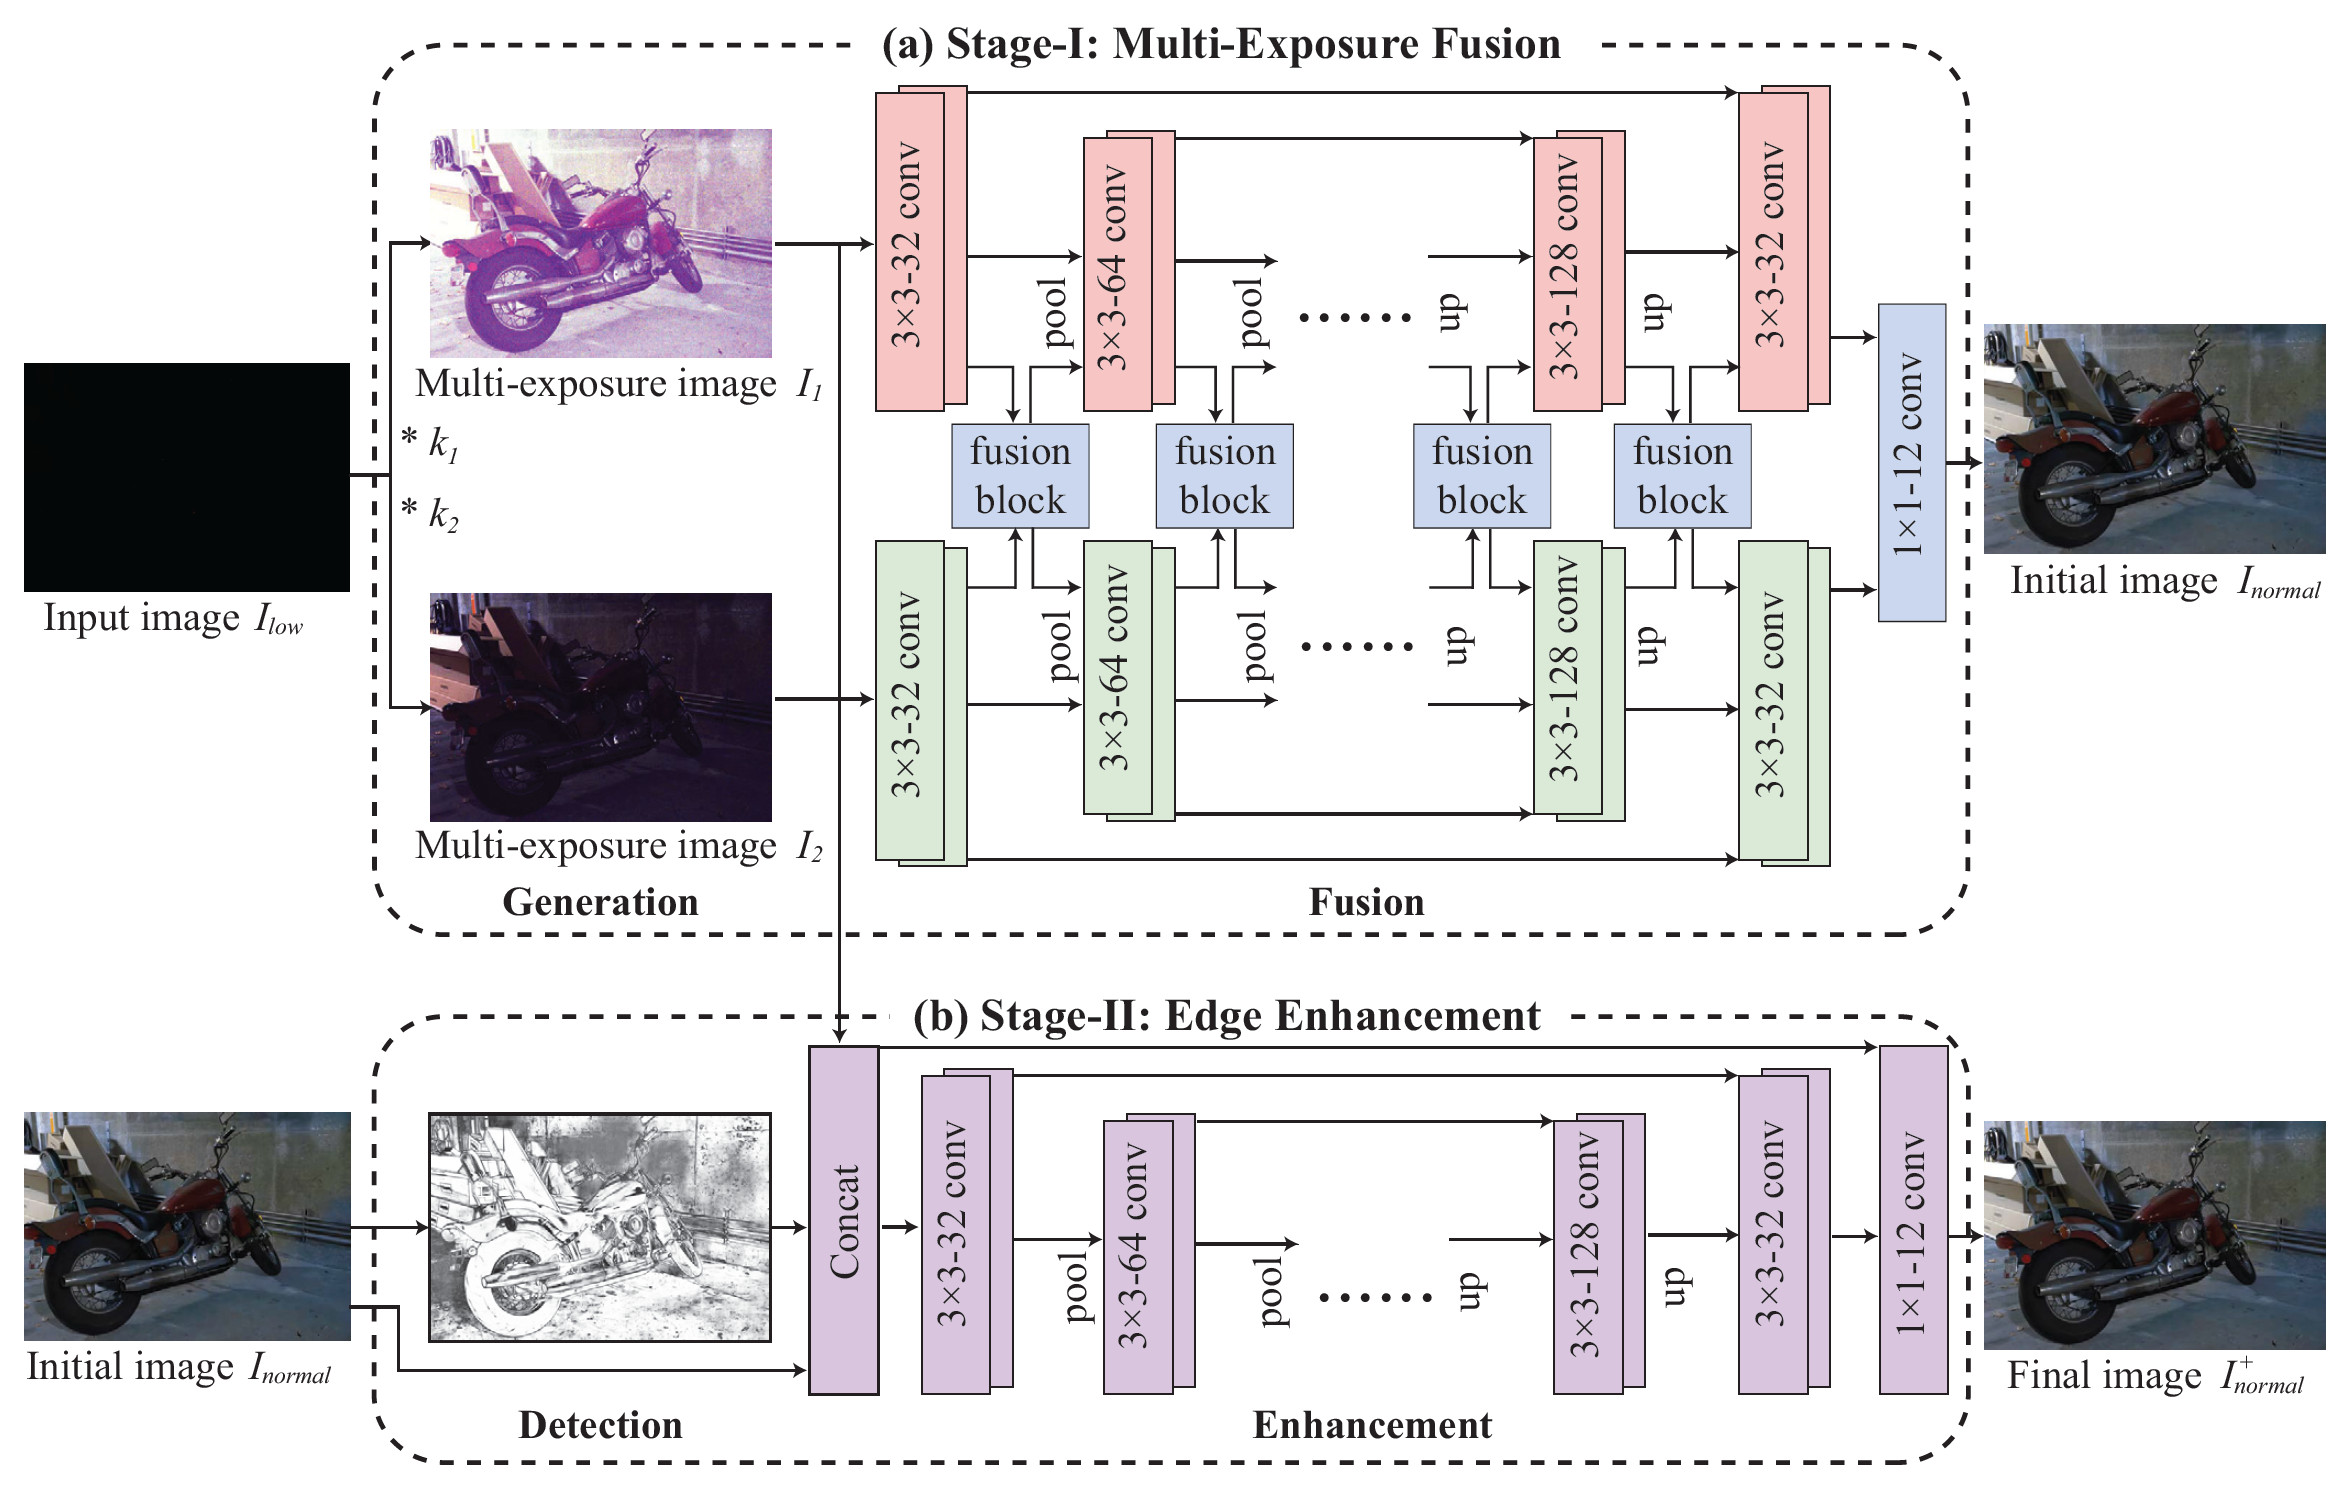
\includegraphics[width=\columnwidth]{picture/LLIE/EEMEFN/EEMEFN framework}
			%\captionsetup{font=scriptsize}
			\caption{
				\label{fig: EEMEFN} 
				该 LLIE 结构源自\cite{zhu2020eemefn},如其 Multi-Exposure Fusion部分采用多曝光融合结构,与由 Initial image 生成的边缘图进行 Concat,后续通过一个 U-Net 网络进一步恢复图像。
			}
		\end{figure}
		
		根据目前的文献调研,当前的此类方法的特点只集中在通过边缘图指导图像恢复,且恢复出来的图像还是有明显噪点。
		
		\subsection{问题一} 
		
		\textbf{图像初步恢复的方法}目前主要包括以下几种:
		
		\begin{itemize}
			\item[(1)] 
			利用多曝光技术\footnote{多曝光技术已被实验证明可以有效的解决 LLIE 任务中普遍存在的色彩失真问题。}获得具有不同曝光度的图像,然后结合恢复网络进行初步恢复\footnote{常见的架构如基于 GAN 的多曝光图像融合架构,基于端到端深度学习框架下多曝光图像融合算法,基于稀疏表示和可平移复方向金字塔变换的多曝光融合框架。};
			
			\item[(2)]
			我们提出的 CNN 和 Transformer 并行架构(见Fig. \ref{fig: First Architecture})。
			
			\item[(3)]
			直接通过神经网络进行弱恢复。
			
		\end{itemize}	
		
		但由于噪声和伪影的存在,以及色彩与真实图像之间的差异,后者结果通常并不理想。

		\subsection{问题二} 
		
		此外,\textbf{获取边缘图的方法}也各不相同,在 LLIE 任务中,常见方法采用\textbf{边缘检测网络}来生成边缘图。Canny 和 Sobel 算子通常被用作对比实验,也有一些研究采用辅助边缘网络以提高边缘图生成的准确性。这些方法在弱光图像恢复研究中都具有一定的学术和实际应用价值。目前在 LLIE 领域中获取边缘图分化成了两个不同的方向,一种是采用初步恢复图像获取边缘图(如Fig. \ref{fig: EEMEFN}),另一种是直接采用弱光图像获取边缘图。
		
		\begin{figure}[htbp]
			% read manual to see what [ht] means and for other possible options
			\centering 
			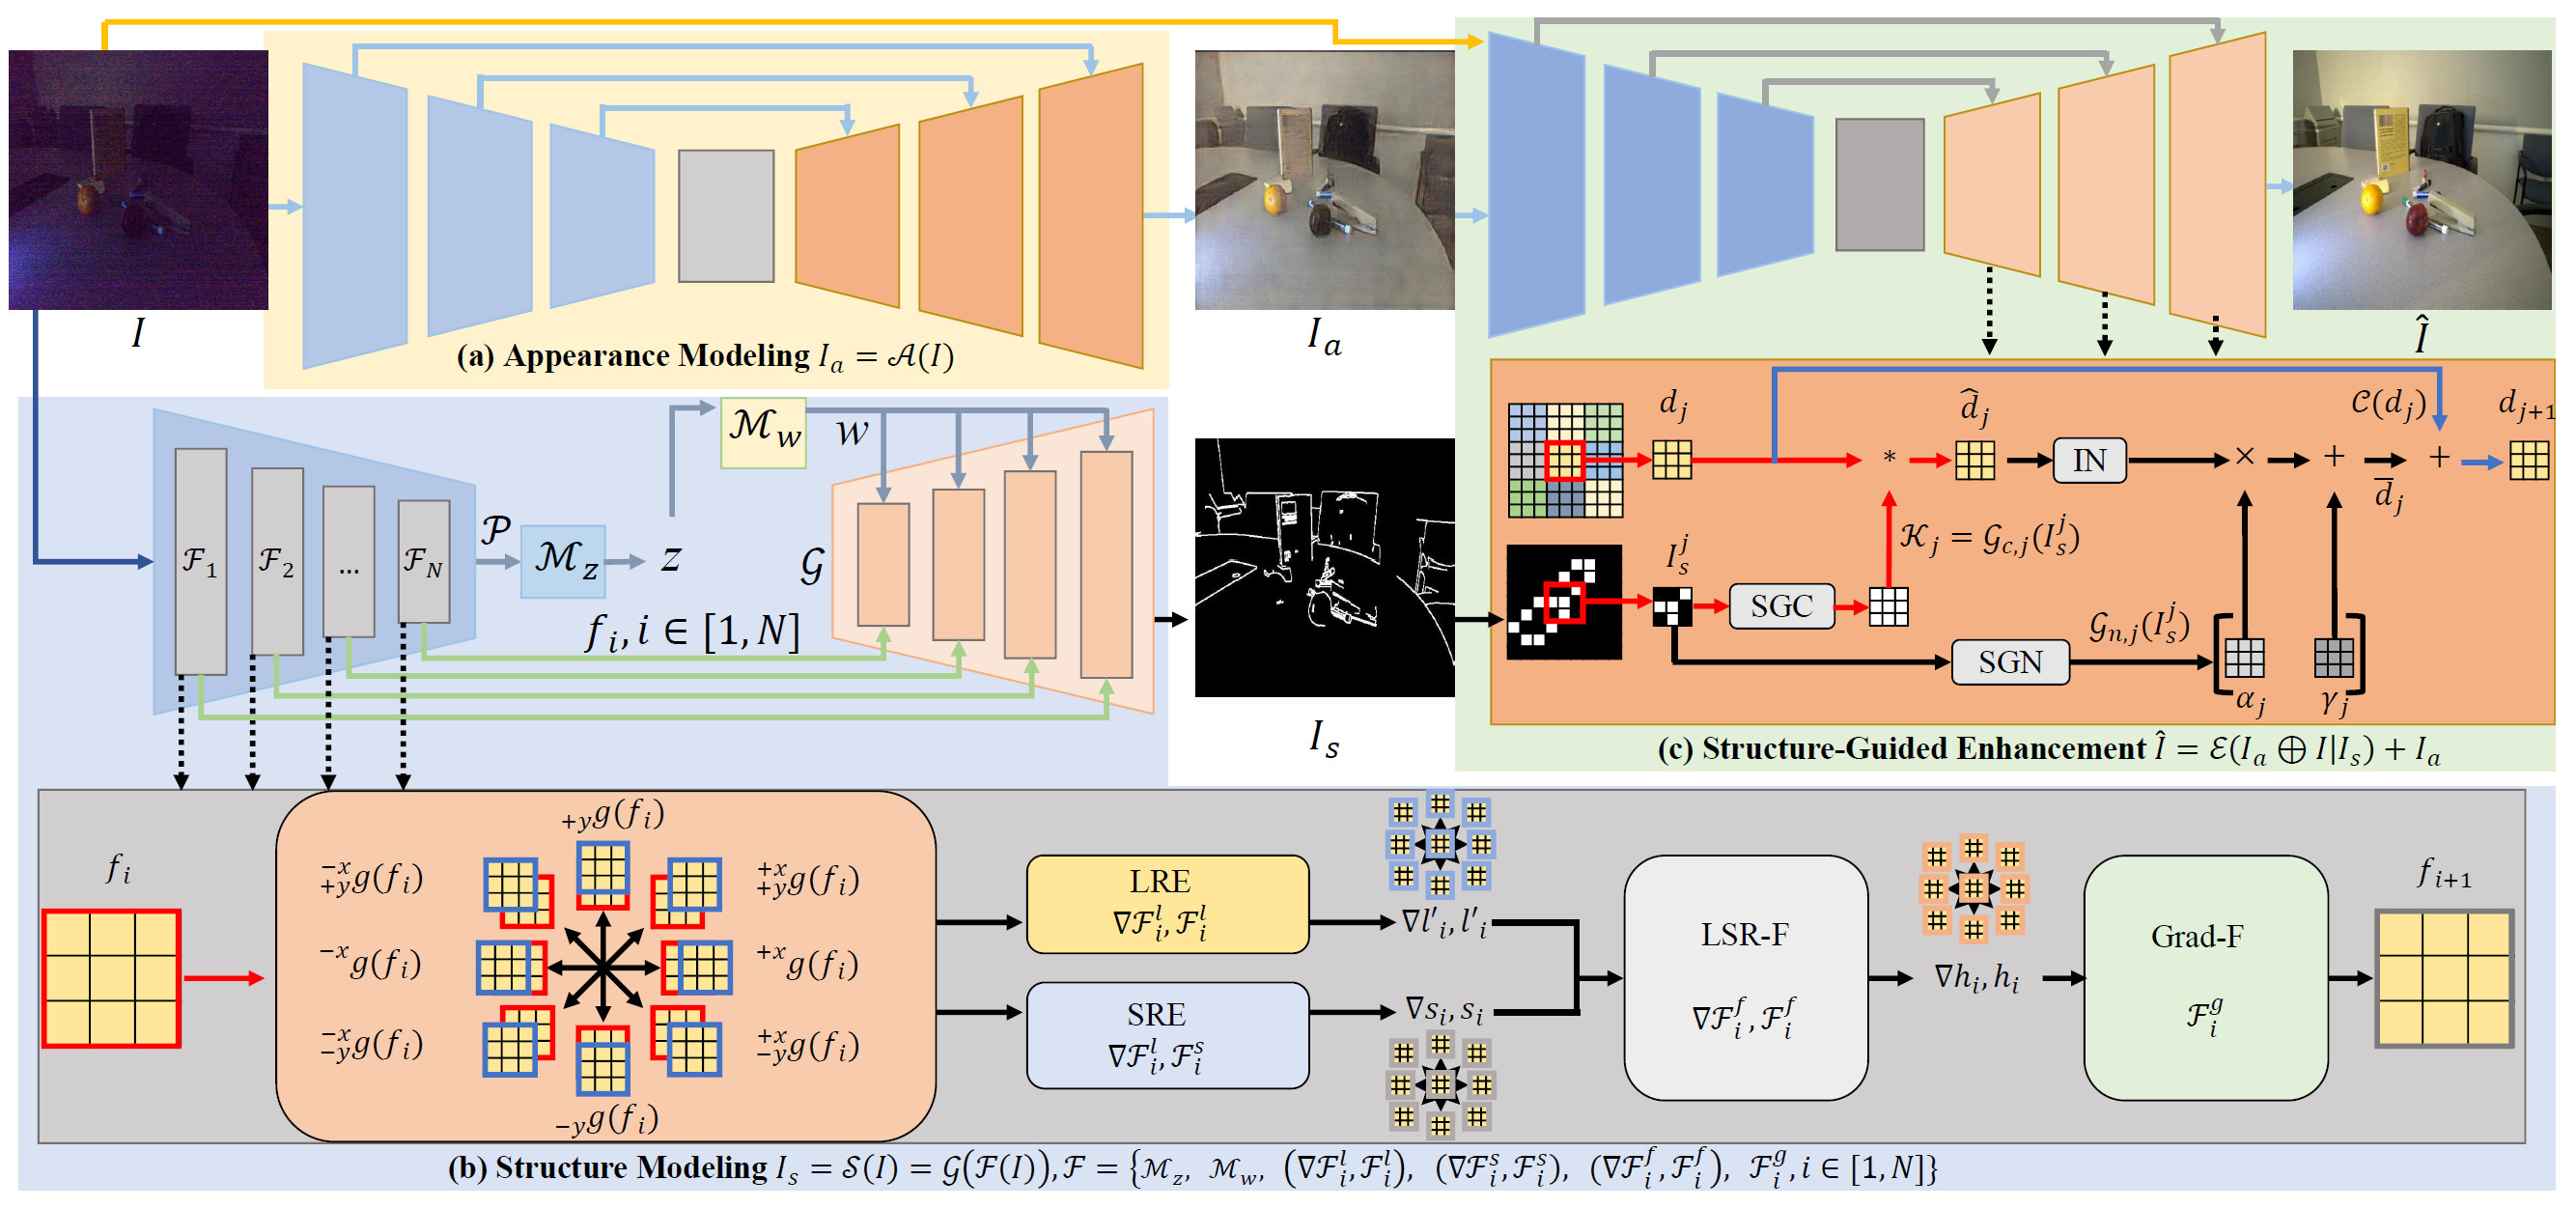
\includegraphics[width=\columnwidth]{picture/LLIE/Structure Modeling and Guidance/Overview}
			%\captionsetup{font=scriptsize}
			\caption{
				\label{fig: Overview} 
				该结构的边缘图直接从 $I$ 中通过 StyleGAN 得到边缘图 $I_s$, 而非从 $I_{\alpha}$ 中通过边缘网络获取边缘图。
			}
		\end{figure}
		
		图像处理任务中边缘检测的各种方法:
		
		\begin{itemize}
			\item[(1)] 
			手工设计各种滤波器来生成边缘图。
			
			\item[(2)]
			根据人类设计的特征使用数据驱动模型来预测边缘(随机决策森林来学习边缘斑块)
			
			\item[(3)]
			深度学习方法从原始数据中学习复杂的特征表示端到端边缘检测模型。
		\end{itemize}	
		
		\subsection{问题三}
		
		在增强网络的设计方面,主要采用了两种主要架构:StyleGAN 和 U-Net。这些网络通常通过串联操作或将边缘图像的分块作为卷积核的方式来引导图像恢复过程。关键点在于边缘图如何为\textbf{初步恢复图片}提供先验增强。
		
	\section{创新想法}
		
		在目前的研究中,我们探索了不同的边缘图生成方法,并引入了基于 VGG 网络的方法,同时采用 Canny 边缘检测作为参考对比方法。我们的主要目标是设计一种综合恢复策略,结合了以下几个关键元素:边缘图、初步恢复图以及原始图像的 Y/Cb/Cr 通道信息。
		
		\begin{figure}[htbp]
			% read manual to see what [ht] means and for other possible options
			\centering 
			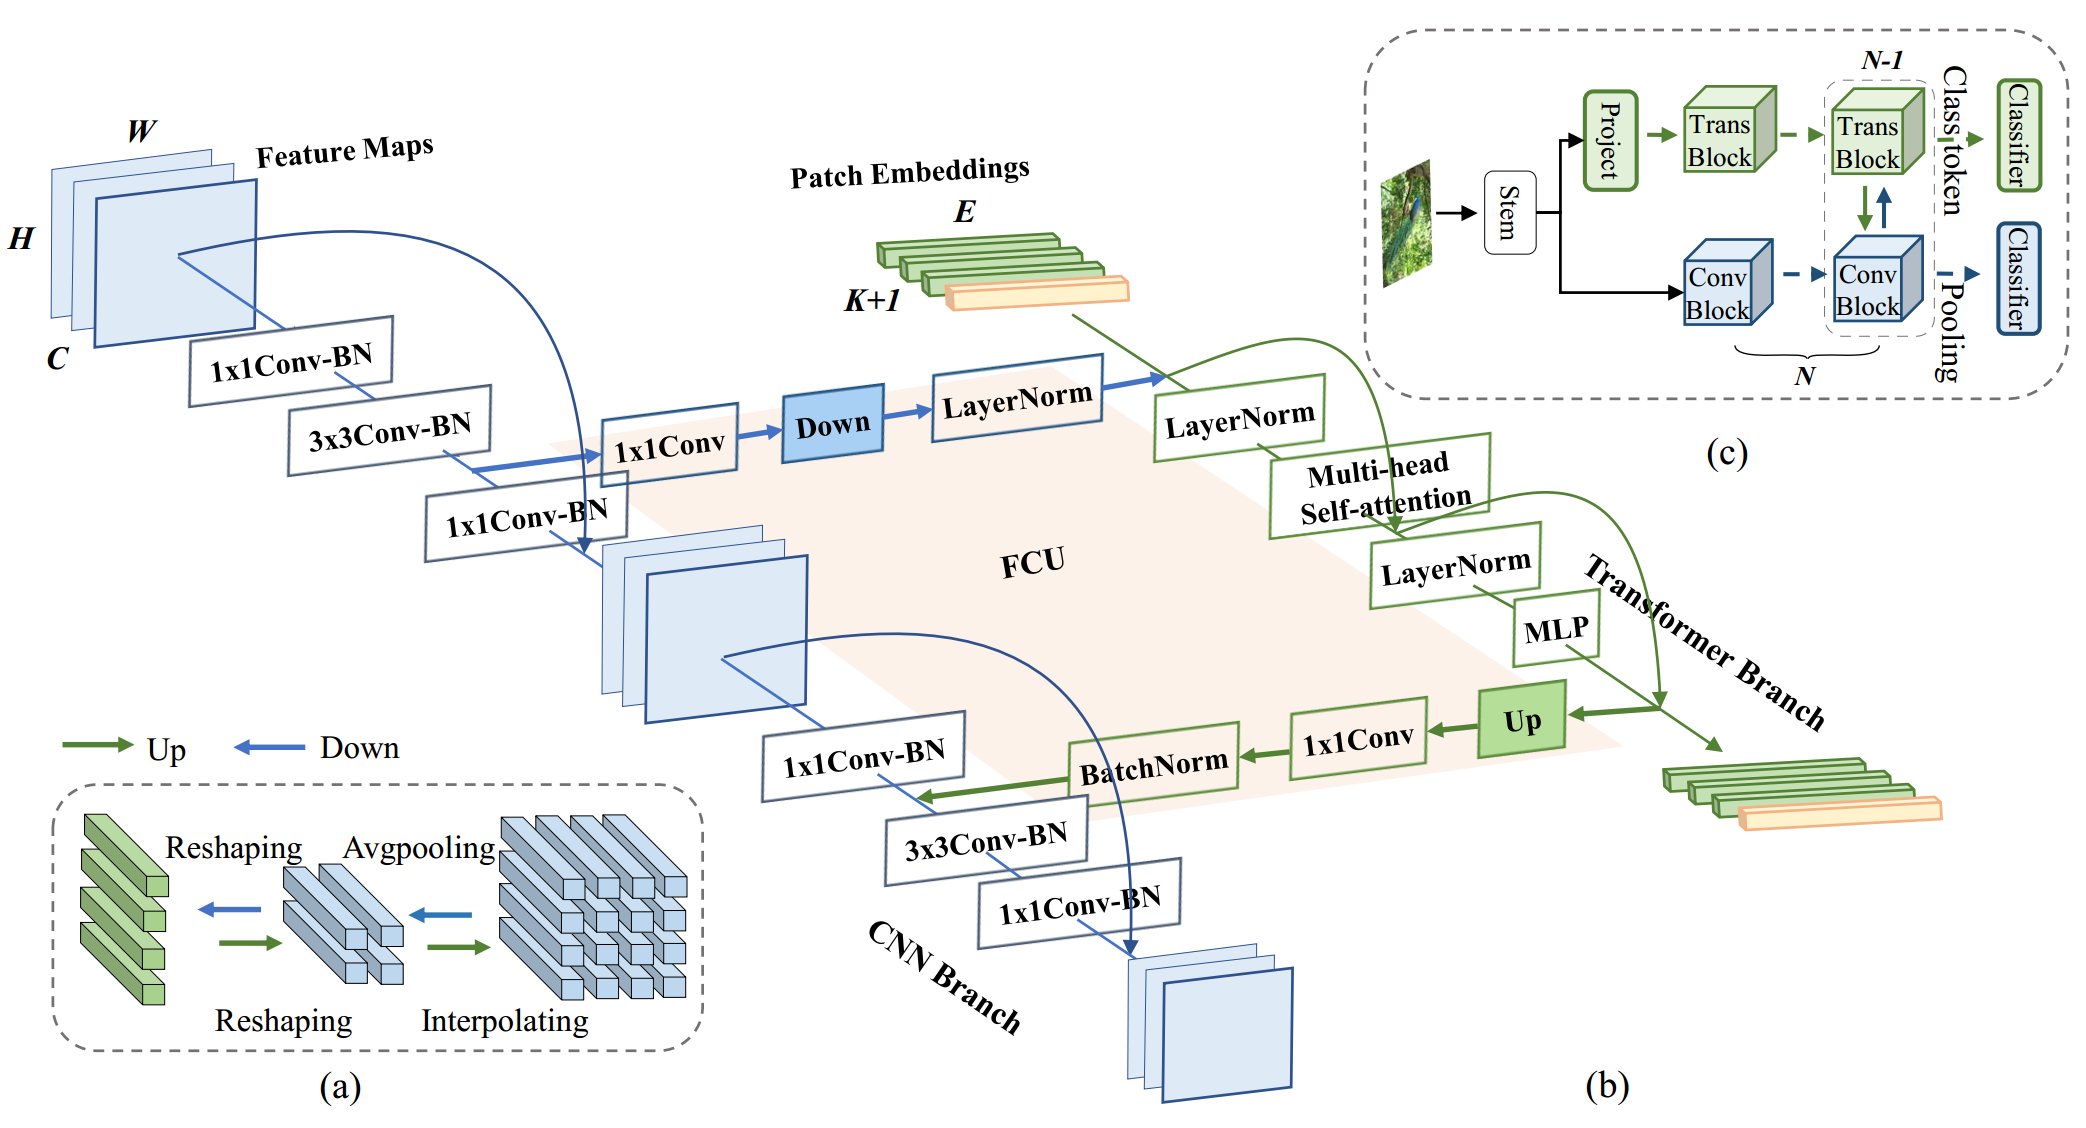
\includegraphics[width=\columnwidth]{picture/LLIE/Conformer/the proposed Conformer}
			%\captionsetup{font=scriptsize}
			\caption{
				\label{fig: Conformer architecture} 
				Network architecture of the proposed Conformer. (a) Up-sampling and down-sampling for spatial alignment of
				feature maps and patch embeddings. (b) Implementation details of the CNN block, the transformer block, and the Feature Coupling Unit (FCU). (c) Thumbnail of Conformer.
			}
		\end{figure}
		
		在初步恢复图的生成方面,我们受到了 Conformer\cite{peng2021conformer} 结构的启发,在卷积神经网络 (CNN) 中,卷积操作擅长提取局部特征,但难以捕获全局表示。Conformer 是一种混合网络结构,包含了并行的 CNN 分支和 Transformer 分支,其通过特征耦合模块融合局部与全局特征,目的在于不损失图像细节的同时捕捉图像全局信息。我们借鉴 Conformer 并发结构 (见 Fig. \ref{fig: Conformer architecture}),将其中 CNN 分支的 ResNet 结构修改为 U-Net 结构(见Fig. \ref{fig: U-Net and AM})。基于这一点,我们设计了一种结合 U-Net 与 Transformer 网络的并行模型 (PACUT, Parallel architecture combining u-net and transformer)(见 Fig. \ref{fig: First Architecture})。这一模型旨在从弱光图像中提取长距离和短距离特征,以便更全面地捕捉图像的信息。通过特定的特征融合策略,我们期望能够得到初步恢复的图像。
		
		至于增强网络的设计,目前计划使用 PACUT 中的 U-Net 改进分支。我们的研究侧重于构建一个整体恢复框架,该框架利用边缘图、初步恢复图和通道信息的融合,以提高弱光图像的质量。我们将继续探索合适的增强网络结构,以便进一步提升恢复结果的性能。这一研究旨在为弱光图像恢复领域提供新的理论和方法,以及改善图像质量并拓展应用领域。
		
		\section{具体实现}
		
		\subsection{Abstract}
		
		在当前的研究中,我们提出了一种新型的深度学习架构,命名为 PACUT ,旨在解决低光照条件下的图像增强问题。该模型结合了经典的U-Net架构和 Transformer 深度学习方法,在弱光图像增强任务中,提高恢复图像的可视性和质量,同时保留重要的细节和纹理信息。
		
		我们提出的 PACUT 模型基于 Conformer 架构,该架构因为在耦合局部特征和全局表示方面的强大潜力而备受欢迎。在 Conformer 中,利用卷积算子提取局部特征,并利用自注意力捕获全局表示,结合特征耦合单元 FCU 来融合局部特征和全局表示,以交互方式增强视觉表示能力。在下游任务中,Conformer显示了成为简单而有效骨干网络的巨大潜力。我们提出的 PACUT 在此基础上进行了以下关键改进:
		
		\begin{itemize}
			
		\item[(1)] 
			深度卷积网络 (CNN) 分支: 该分支基于 U-Net 架构,采用多层卷积神经网络,通过逐层提取图像的局部特征来增强图像的细节和纹理。此分支的设计旨在处理图像的低级特征,如边缘、纹理和颜色信息。
			
		\item[(2)]
			Vision Transformer (ViT) 分支: 该分支利用了 Vision Transformer 的能力,通过自注意力机制捕捉图像的长距离依赖关系。ViT分支专注于提取图像的全局特征,如整体结构和上下文信息。
			
		\item[(3)]
			特征耦合单元 (FCU): 为了有效地融合 CNN 分支和 ViT 分支的特征,引入了特征耦合单元 (FCU)。FCU 通过下采样 (FCUDown) 和上采样 (FCUUp) 操作,实现了 CNN特征图和 Transformer patch embeddings 之间的无缝转换,从而实现了局部特征和全局表示的连续耦合。
			
		\end{itemize}
		
		
		PACUT 模型在低光照图像增强领域展现出巨大潜力。其能够有效提升图像的亮度和对比度,同时保留关键细节,适用于监控、医学成像、天文观测等领域。此外,该模型的设计理念也可推广应用于其他图像处理任务,如图像去噪、超分辨率和风格迁移。我们在弱光图像增强任务中,创新性地提出了并行特征耦合策略,为深度学习在 LLIE 任务中的应用提供了一种全新的视角。
		
		\subsection{PACUT Architecture}
		
		在计算机视觉领域,我们往往研究图像的两种主要特征:局部特征和全局表征。局部特征\cite{jain1991unsupervised}\cite{lowe2004distinctive}\cite{ojala2002multiresolution}是对图像中小区域的紧凑向量描述,它们是许多计算机视觉算法的基础。而全局表征则包括更宽范围的特征,比如长距离的轮廓\cite{lisin2005combining}、形状描述符以及不同对象的类型。在深度学习的背景下,卷积神经网络 (CNN) 通过层级的卷积操作,逐层提取图像的局部特征,并将这些特征保留在特征图中。而视觉变换器则通过一系列自我关注的模块,以一种更加灵活的方式,将这些特征聚合起来,形成对整体图像的全局理解。
		
		为了充分利用局部特征和全局表征,我们设计了一种并行网络结构,如Fig. \ref{fig: The proposed initial architecture(Abstract Picture)}所示,称为 PACUT (Parallel architecture combining u-net and transformer)。考虑到这两种模型风格特征的互补性,在 PACUT 中,我们通过一个交互过程以互补两种模型的优劣,将 Transformer 分支的全局上下文连续输入到特征图中,以增强卷积神经网络 (CNN) 分支的全局感知能力。同样,CNN 分支的局部特征逐步反馈到 Patch Embedding 中,以丰富 Transformer 分支的局部细节。
		
		\begin{figure}[htb] 
			% read manual to see what [ht] means and for other possible options
			\centering 
			% 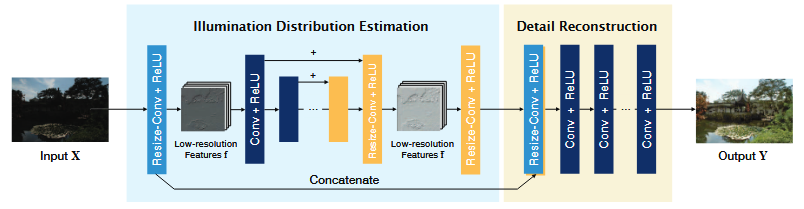
\includegraphics[width=0.8\columnwidth]{GLADNet}
			
			\begin{subfigure}{\textwidth}
				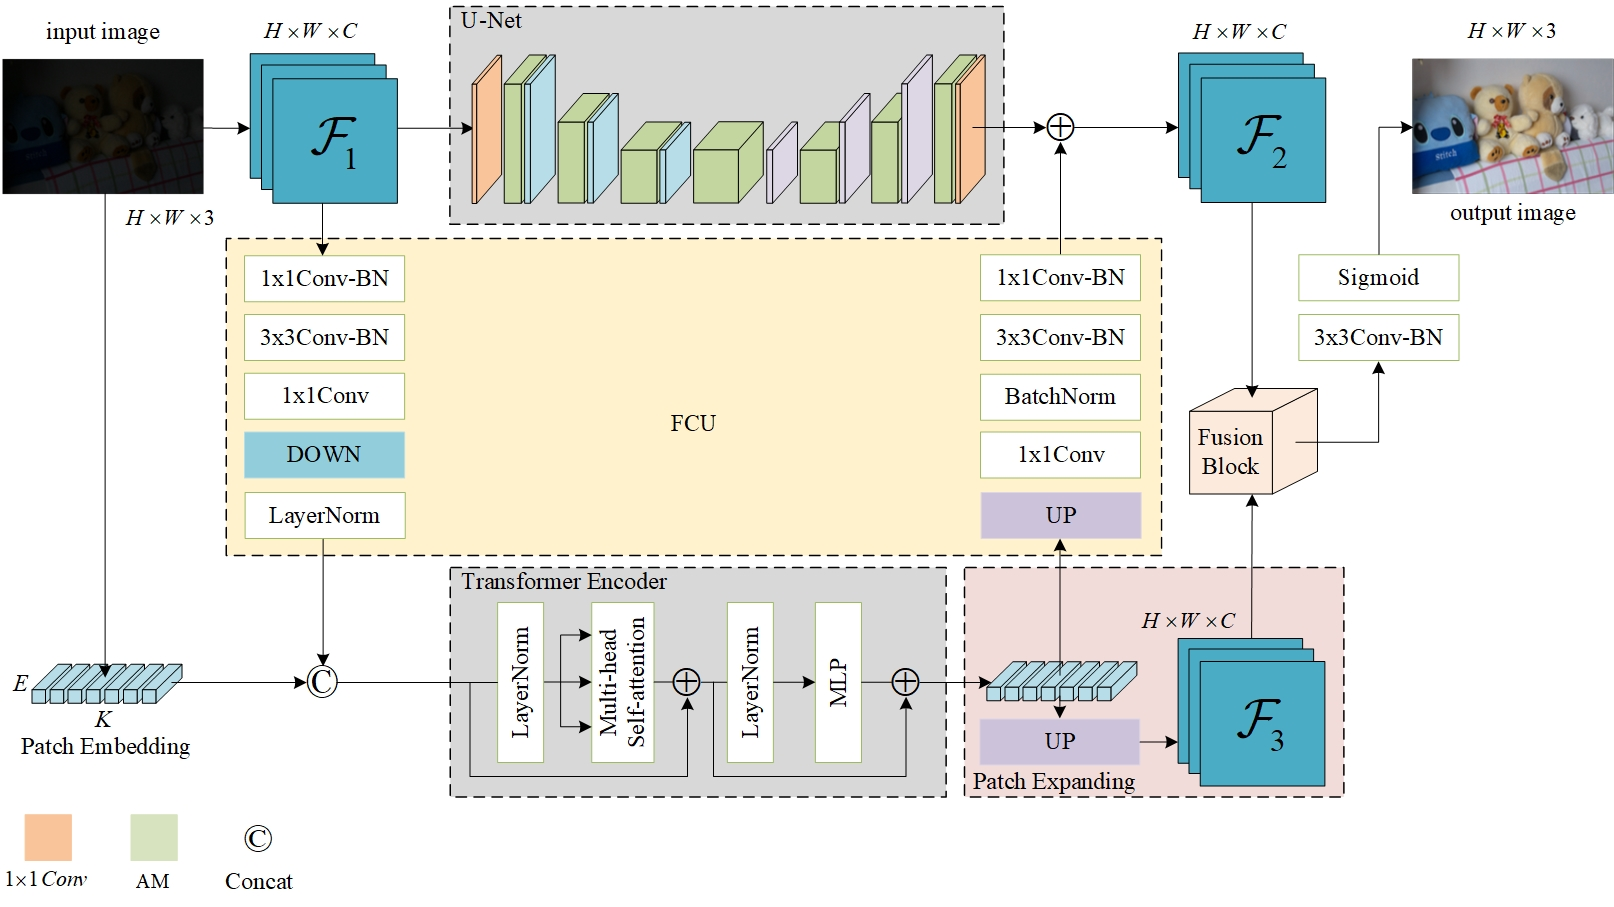
\includegraphics[width=\linewidth]{picture/LLIE/My Architecture/The proposed initial architecture.jpg}
				\captionsetup{font=scriptsize}
				\caption{PACUT}
				\label{fig: First Architecture}
			\end{subfigure}\\
			\begin{subfigure}{0.4\textwidth}
				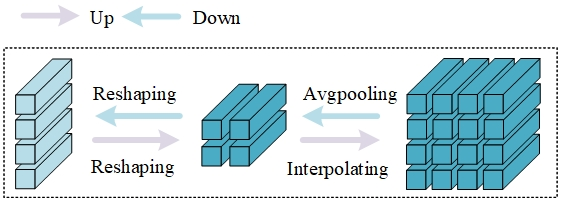
\includegraphics[width=\linewidth]{picture/LLIE/My Architecture/Up-sampling and down-sampling}
				\captionsetup{font=scriptsize}
				\caption{Up-sampling and Down-sampling}
				\label{fig: Up-sampling and down-sampling}
			\end{subfigure} \
			\begin{subfigure}{0.4\textwidth}
				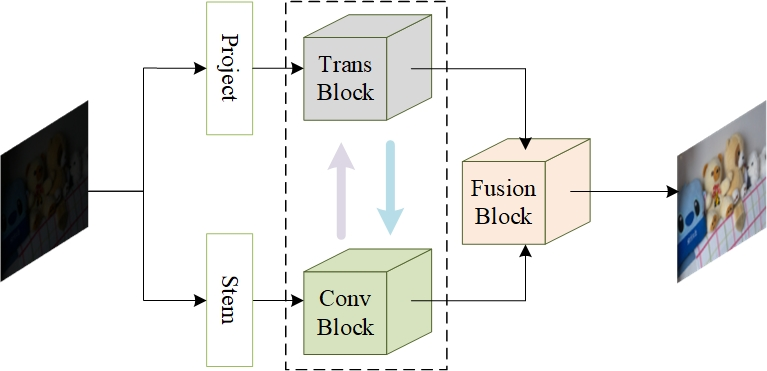
\includegraphics[width=\linewidth]{picture/LLIE/My Architecture/The proposed initial architecture(Abstract Picture)}
				\captionsetup{font=scriptsize}
				\caption{Thumbnail of PACUT}
				\label{fig: The proposed initial architecture(Abstract Picture)}	
			\end{subfigure}
			
			\captionsetup{font=scriptsize}
			\caption{
				\label{fig: PACUT}
				PACUT 模型结构。Fig. \ref{fig: First Architecture} CNN 分支和 Transformer 分支以及 FCU (Feature Coupling Unit)。Fig. \ref{fig: Up-sampling and down-sampling} 特征映射和 Patch embeddings 空间对齐的上采样和下采样过程。 Fig. \ref{fig: The proposed initial architecture(Abstract Picture)} PACUT 的缩略图。PACUT 结构受 Conformer\cite{peng2021conformer} (见 Fig. \ref{fig: Conformer architecture})启发,将原来结构中 CNN 分支的 ResNet 结构修改为 U-Net 结构。其采用一个 U-Net 和 ViT 的并行架构,通过 U-Net 结构得到一个弱恢复的弱特征图 $\mathcal{F}_2$,通过 ViT 融合的特征可以初步增强弱特征图 $\mathcal{F}_2$,ViT 的输出经过 Patch Expanding 的特征图 $\mathcal{F}_3$ 经过与 U-Net 输出的特征图 $\mathcal{F}_2$ 融合之后得到一个初步恢复的图片 output image,用以后续参与图片的进一步恢复。
			}
		\end{figure}
		
		详细地说,PACUT 由双分支、Stem 模块、用于连接双分支的特征连接单元 (FCU, Feature Coupling Unit),以及为双分支设计的一个融合模块 (Fusion Block) 组成。Stem 模块由 VGG16 网络的前四层组成,截至第一个最大池化层,用于提取图像的初始局部特征,如边缘、纹理等,然后将其输入到 CNN 分支。
%		我们通过以下步骤实现了这一结构:首先,加载预训练的 VGG16 模型;随后,利用 PyTorch 框架中的 nn.Sequential 方法,将 VGG16 的特征层 (vgg.features) 转换为一个序列,并选择这个序列的前四个子层作为我们的 Stem 模块。
		Stem 模块的主要作用是提取图像的初始局部特征,如边缘、纹理等。CNN 分支是一种改进的 U-Net 网络结构,Transformer 分支由 去掉分类功能只保留特征提取功能的 Vision Transformer 结构组成。 
		
		这样的并行结构意味着CNN分支和变换器分支分别能够最大限度地保留局部特征和全局表征。我们提出 FCU 作为一种桥接模块,用于融合CNN分支中的局部特征和变换器分支中的全局表征,如 Fig. \ref{fig: First Architecture} 所示。 FCU 从第二步开始应用,因为两个分支的初始特征是相同的,只是表征形式不同。沿着分支,FCU 通过两个来回式的交互融合特征图和 Patch Embeddings。
		
		最后,两个分支的特征都被输入到特征融合模块中。对于 Transformer 分支,我们为了更好的利用获取的长距离特征,在进行 Patch Expanding 操作之前,通过 FCU 与 CNN 分支融合。最后两个分支通过特征融合模块处理后获取增强图像。在训练过程中,我们结合 $\mathcal{L}_1$ 和 SSIM 损失函数来同时优化模型在像素级误差和感知质量方面的表现。

		
		\subsubsection{CNN Branch}	
			
		CNN 分支的基础是 U-Net 结构,这是一种专门为图像分割任务设计的网络架构,但在图像增强领域也表现出色。U-Net 的特点是其对称的编码器-解码器结构,以及编码器和解码器之间的跳跃连接。CNN 分支的目标是从输入的弱光图像 (LLI) 中提取丰富的特征,包括边缘、纹理、颜色、亮度信息,并最终输出增强的图像 (EI)。
		
		\paragraph{UNetEnhance}
		
		UNetEnhance 模型是一种针对低光照图像增强任务设计的深度学习架构。该模型基于经典的 U-Net 架构,并引入了多项改进,以提高对低光照环境下图像的处理能力。这些改进包括更深的网络结构、改进的特征融合机制和高效的信息传递路径。
		
		\begin{figure}[htb]
			% read manual to see what [ht] means and for other possible options
			\centering 
			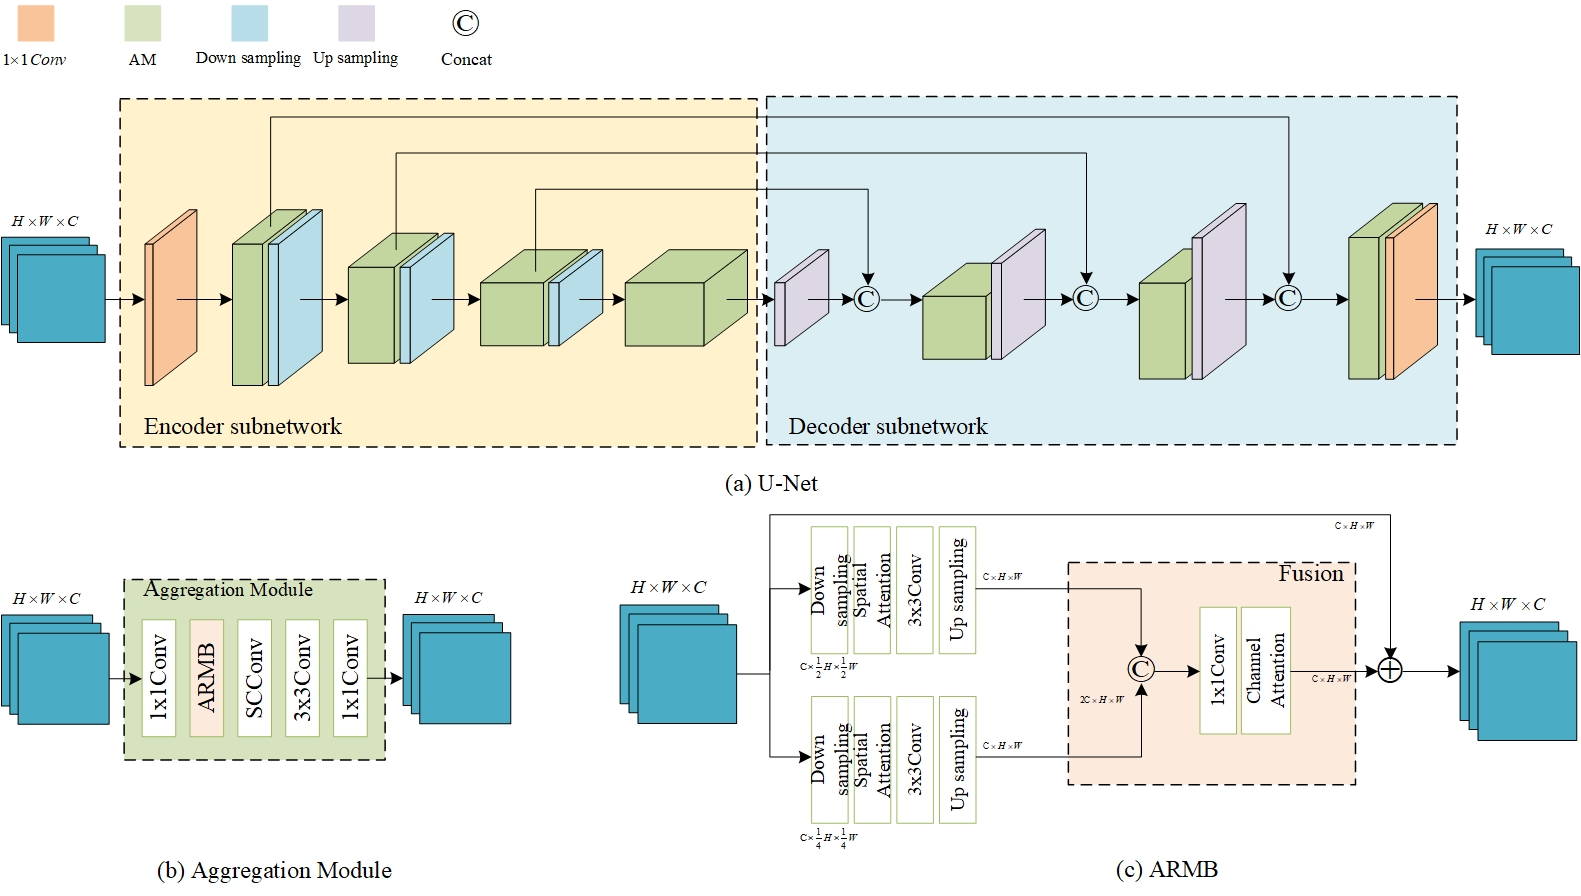
\includegraphics[width=\columnwidth]{picture/LLIE/My Architecture/U-Net and AM}
			%\captionsetup{font=scriptsize}
			\caption{
				\label{fig: U-Net and AM} 
				U-Net 图像初步恢复网络及其所属的模块。
			}
		\end{figure}
		
		我们提出的 UNetEnhance 模型如 Fig. \ref{fig: U-Net and AM} 所示,它由两个部分组成:1) 编码器子网络 (Encoder subnetworker),2) 解码器子网络 (Decoder subnetworker)。对于编码器子网络,UNetEnhance 采用了多层卷积网络,在每层中我们添加了集成模块,在集成模块中又添加了空间注意力机制和通道注意力机制\cite{woo2018cbam}。与传统 U-Net 相比,这一设计增加了网络的深度,从而能够捕获更加丰富的特征信息。我们通过引入更多的卷积层,使得模型能够在更深的层次上理解图像内容。解码器部分采用了上采样和卷积操作,以逐步恢复图像的空间分辨率。在这一过程中,引入了改进的特征融合策略,将编码器中的低级特征与解码器的高级特征有效结合,从而更好地重建图像细节。同时,UNetEnhance 模型在跳跃连接的设计上进行了优化,以更有效地传递编码器中的特征信息到编码器。这些连接不仅帮助保留了在下采样过程中可能丢失的细节信息,还增强了网络的特征重建能力。此外,模型的输出层经过特别设计,以确保输出图像在视觉上的质量和连贯性,我们通过准确的调整解码器子网络中的卷积操作,将解码器的输出转换为与原始输入图像相同尺寸的增强图像。
		
		假设 $I_{LLI}$ 表示输入的弱光图像,$I_{EI}$ 表示输出的增强图像。编码器子网络 $\mathcal{E}$ 和解码器子网络 $\mathcal{D}$ 的操作可以表示为:
		
		\begin{equation}
			\begin{aligned}
				I_{EI} = \mathcal{D} \left( \mathcal{E} \left( I_{LLI} \right) \right)
			\end{aligned}
			\label{eq: UNetEnhance model}
		\end{equation}
		
		对于 AM 集成模块(Fig. \ref{fig: U-Net and AM}b),其操作可表示为:
		
		\begin{equation}
			\begin{aligned}
				\text{AM}_{i}(x) = f^{1 \times 1} \left(f^{3 \times 3} \left(\text{SCConv}\left( \text{ARMB} \left( f^{1 \times 1} (x)\right)\right)\right)\right)
			\end{aligned}
			\label{eq: Aggregation Module}
		\end{equation}
		
		其中,$f^{1\times1}$为 $1 \times 1$ 卷积层,ARMB 和 SCConv 的操作依据其内部结构进行。
		
		编码器首先通过一个 $1 \times 1$ 卷积层处理输入图像,用于提取初始特征。然后连续通过四个单元,前三个单元每一个都由一个 AM 集成模块 $\text{AM}_i$ 和一个池化层组成,第四个单元仅包含一个 AM 集成模块。AM 集成模块由一系列卷积层和特殊的注意力机制组成的复杂结构,包括 ARMB 模块和 SCConv 模块,见 Eq. \ref{eq: Aggregation Module}。
		
		解码器首先通过一个上采样模块,然后与 $\text{AM}_{3}$ 进行拼接操作,然后通过 $\text{AM}_{5}$ 集成模块和上采样模块,然后与 $\text{AM}_{2}$ 拼接,然后通过 $\text{AM}_{6}$ 集成模块和上采样模块,然后与 $\text{AM}_{1}$ 拼接,最后通过 $\text{AM}_{7}$ 集成模块和 $1 \times 1$ 卷积层。
		
		\paragraph{Attentive Residual Multiscale Block}
		
		ARMB (Attention Residual Merging Block) 是一种用于深度学习模型中的结构单元,特别是在处理图像相关任务时,它的主要作用是融合来自不同来源的特征,并通过注意力机制增强模型对关键信息的关注。其核心作用之一是融合来自模型不同层或不同分支的特征。这种融合有助于结合低级特征(如边缘和纹理)和高级特征(如对象部分和语义信息),从而提升模型的表现力。ARMB 中的注意力机制有助于 UNetEnhance 更加关注于图像中的重要区域或特征。通过加权重要特征,ARMB 可以提高模型对关键信息的敏感性。ARMB 通过残差连接来解决深度神经网络中的梯度消失问题。如Fig .\ref{fig: U-Net and AM}c 所示,残差连接允许信息直接从早期层传递到后续层,从而保持信息流的连续性。
		
		模块对输入特征 $\mathcal{F}$ 进行两次分支下采样,分别获取尺寸为 $\frac{1}{2}$ 和 $\frac{1}{4}$ 的特征。每个分支使用空间注意力 (Spatial Attention) 过滤噪声,通过 $3 \times 3$ 卷积层提取特征,并通过上采样恢复到原始尺寸。将两个特征图拼接后,通过$ 1 \times 1$ 卷积层处理,再应用通道注意力 (Channel Attention) 进行特征加权,最后通过跳跃连接与原始输 $\mathcal{F}$ 合并,得到最终特征图。
		
		假设 $\mathcal{F}_{in}$ 是输入特征图,$\mathcal{F}_{out}$ 是输出特征图,$\mathcal{F}_{i}^\prime$ 表示对特征图进行裁剪或放大,见下式:
		
		\begin{equation}
			\begin{aligned}
				&\mathcal{F}^\prime_{\frac{1}{2}} = \text{Resize}\left(\mathcal{F}_{in},\left(\frac{H}{2},\frac{W}{2}\right)\right), \\
				&\mathcal{F}^\prime_{\frac{1}{4}} = \text{Resize}\left(\mathcal{F}_{in},\left(\frac{H}{4},\frac{W}{4}\right)\right), \\
				&\mathcal{F}_{out} = W_1\mathcal{F}_{out} + W_2\mathcal{C} \left( f^{1 \times 1}  \left[\mathcal{F}^\prime_2 (f^{3 \times 3}(\mathcal{S}(\mathcal{F}^\prime_{\frac{1}{2}}))), \mathcal{F}^\prime_4 (f^{3 \times 3}(\mathcal{S}(\mathcal{F}^\prime_{\frac{1}{4}})))\right] \right).
			\end{aligned}
			\label{eq: ARMB}
		\end{equation}
		
		其中 $\mathcal{S}$ 和 $\mathcal{C}$ 分别表示空间注意力函数和通道注意力函数,$W_1$ 和 $W_2$ 为对应的特征图权重。
		
		\paragraph{SCConv}
		
		SCConv 模块是一种用于特征冗余的空间和通道重构卷积,由 SRU 和 CRU 两个子模块组成。SRU 用于通过门控机制选择性地激活特征,而 CRU 负责特征的融合和重构。
		
		\subsubsection{Transformer Branch}
		
		Transformer 分支主要基于 Vision Transformer (ViT) 架构,用于从图像中提取全局特征。这一分支的目标是捕获图像中的长距离依赖关系,以辅助 CNN 分支的局部特征提取。
		
		\paragraph{Patch Embedding}
		
		在深度学习和计算机视觉中,Patch Embedding 是一种常见的操作,它将图像分割成更小的块 (patches),然后将这些块转换成一系列的向量,这些向量可以被用作模型的输入。
		
		\begin{figure}[htb]
			% read manual to see what [ht] means and for other possible options
			\centering 
			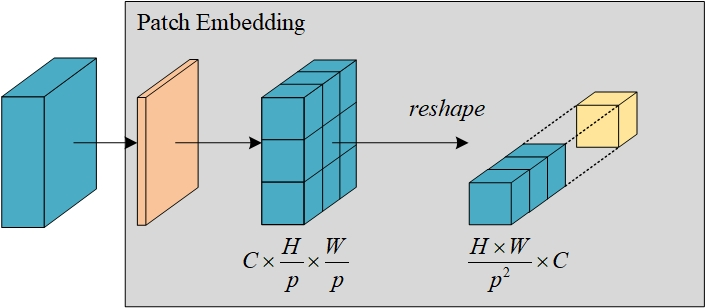
\includegraphics[width=0.5\columnwidth]{picture/LLIE/My Architecture/Patch Embedding}
			%\captionsetup{font=scriptsize}
			\caption{
				\label{fig: Patch Embedding} 
				Patch Embedding 的一般性过程。
			}
		\end{figure}
		
		首先,对原始的弱光图像 $P_1$ 压缩尺寸至固定尺寸,以匹配预训练 Vision Transformer 模型的权重。对 LLI 进行 Patch Embedding,得到 576 个 D 维的特征向量,每个向量对应于一个 $16 \times 16$ 的 patch。然后,将 $384 \times 384$ 的特征向量重新排列成 576 个 $16 \times 16$的 patches,然后每个 patch 也被 flatten 成 256 维的向量。因为是三通道特征,所以实际上每个通道被 flatten 成 256 维,总计 $256 \times 3$ 维的向量 $\ell_1$。
		
		\begin{figure}[htb]
			% read manual to see what [ht] means and for other possible options
			\centering 
			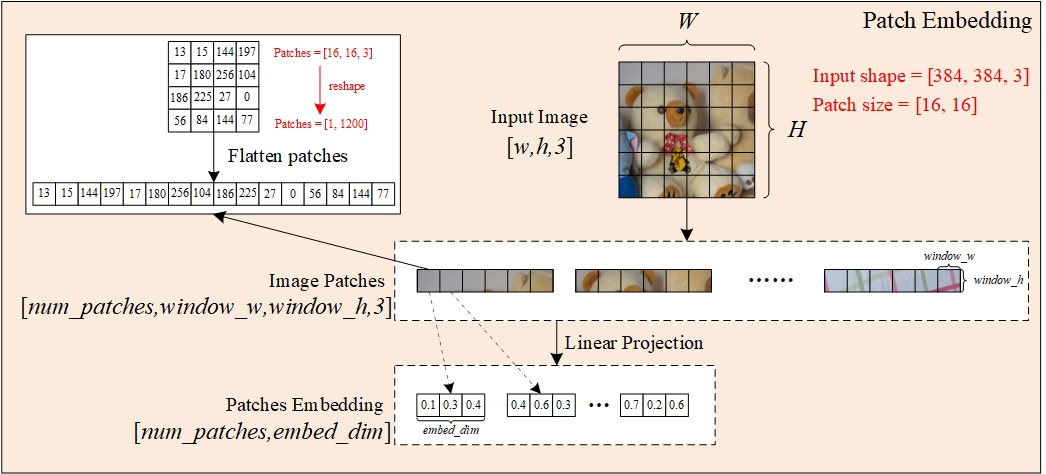
\includegraphics[width=0.8\columnwidth]{picture/LLIE/My Architecture/Patch Embedding(ViT)}
			%\captionsetup{font=scriptsize}
			\caption{
				\label{fig: Patch Embedding(ViT)} 
				Transformer 分支中 Patch Embedding 的过程。
			}
		\end{figure}
		
		实际上,我们可以将 $\ell_1$ 通过一个 Linear Projection,使其转换成 D 维的向量,如 Fig. \ref{fig: Patch Embedding(ViT)} 所示。
		
		Patch Embedding 的具体过程可以被描述为下列过程:
		
		\begin{itemize}
			\item[$\bullet$] 
			输入图像 $X \in \mathbb{R}^{H \times W \times C}$,其中 $H$,$W$和$C$ 分别代表图像的高度、宽度和通道数。
			\item[$\bullet$]
			图像被分割成 $N$ 个大小为 $P \times P$ 的 patches,每个 patch 被展平并线性投影到 D 维空间,得到 patch embeddings $E \in \mathbb{R}^{N \times D}$
		\end{itemize}
		
		Fig. \ref{fig: First Architecture} 显示了在 Patech Embedding 之后,会将特征 $\mathcal{F}_1$ 进行变换处理之后与向量 $\ell_1$ 进行 Concat 操作(不经过处理特征 $\mathcal{F}_1$ 无法直接与向量 $\ell_1$ 拼接)。
		
		使用 $20 \times 20$ 的 Patch 大小进行 Embedding,但是这个大小是否合适取决于输入图像的尺寸和细节的重要性。如果图像中包含细小的重要特征,较小的 Patch 可能更合适。另一方面,较大的 Patch 可能会捕捉到更高层次的抽象特征。后续可能需要实验不同的 Patch 大小来找到最佳的平衡点。
		
		\paragraph{Positional Encoding}
		
		在Transformer中,由于缺乏像卷积神经网络 (CNN) 那样的固有空间结构,需要一种方法来告知模型不同 patches 之间的相对或绝对位置。Positional Encoding就是为了解决这个问题而设计的。
		
		Positional Encoding 通常是通过将一个固定的或可学习的编码添加到每个 patch 的 embedding 中来实现的。这个编码是根据 patch 在原始图像中的位置计算得出的。一种常见的方法是使用正弦和余弦函数的组合来生成每个位置的编码。例如,对于位置 pos 和维度 i,编码可以计算为:
		
		\begin{equation}
			\begin{aligned}
				&\text{PE}(\text{pos}, \ 2i) = \sin \left(\frac{\text{pos}}{10000^{\frac{2i}{D}}}\right) \\
				&\text{PE}(\text{pos}, \ 2i + 1) = \cos \left(\frac{\text{pos}}{10000^{\frac{2i}{D}}}\right)
			\end{aligned}
			\label{eq: positional encoding}
		\end{equation}
		
		其中,D 是 embedding 的维度。计算出的 Positional Encoding 被加到每个 patch 的 embedding 上。位置编码为 $PE \in \mathbb{R}^{N \times D}$,Positional Encoding 被描述为 $E_{pos} = E + PE$。 这样,即使在多头自注意力机制中,模型也能够利用这些编码来理解和利用 patches 之间的相对位置信息。在ViT中,Positional Encoding对于模型理解图像内容至关重要。它允许模型捕捉到图像中的空间层次结构和对象之间的相对位置关系,这对于图像理解任务来说是非常重要的。
		
		我们采用 timm 库来创建预训练的ViT模型,并移除了原始的分类头,在 timm 库中创建的预训练 ViT 模型已经内置了Positional Encoding的过程。
		
		\paragraph{Transformer Encoder}
		
		在Vision Transformer (ViT) 架构中,Transformer Encoder 是核心组件,负责处理图像的序列化表示。经过位置编码的 Patch Embeddings 被送入 Transformer 的编码器。如 Fig. \ref{fig: First Architecture} 所示,Transformer 编码器主要设计两个主要步骤,包括多头自注意力机制 (Multi-head Self-Attention) 和多层感知器 (Multi-Layer Perceptron)。这些组件共同工作,以捕获图像中的复杂特征和长距离依赖关系。
		
		其中,多头自注意力机制允许模型在处理每个图像 patch 时同时考虑其他所有 patch 的信息。通过这种方式,模型能够捕获图像中不同区域之间的复杂关系和依赖性。在多头自注意力中,注意力机制被分割成多个“头”,每个头学习图像的不同方面,从而提高了模型的表达能力。MLP 由多个线性层和非线性激活函数组成,它为模型引入了必要的非线性处理能力。这种非线性是处理复杂数据(如图像)时不可或缺的,因为它允许模型学习更加复杂和抽象的特征表示。
		
		对于每个 Transformer 层 $l$,输入 $X_l$ 经过以下过程:
		
		\begin{itemize}
			\item[1)] 
			多头自注意力 (MSA):
			\begin{equation}
				\begin{aligned}
					\text{MSA}(X_l) = [\text{head}_1, \text{head}_2, \ldots, \text{head}_k] W^{O}
				\end{aligned}
				\label{eq: MSA}
			\end{equation}
			其中每个 head 是 $\text{head}_i = \text{Attention}\left(X_l W_i^Q, X_l W_i^K, X_l W_i^V \right)$。Attention 机制通常定义为
			\begin{equation}
				\begin{aligned}
					\text{Attention}(Q, K, V) = \text{softmax} \left(\frac{QK^T}{\sqrt{d_k}} \right) V
				\end{aligned}
				\label{eq: Attention}
			\end{equation}
			其中 $d_k$ 是 key 向量的维度。
				
			\item[2)]
			残差连接和层归一化:
			\begin{equation}
				\begin{aligned}
					X_l^\prime = \text{LayerNorm} \left(X_l + \text{MSA}(X_l)\right)
				\end{aligned}
				\label{eq: MSA}
			\end{equation}
			\item[3)]
			多层感知机:
			
			MLP 包含两个全连接层和一个激活函数,即 $\text{MLP} (X_l^\prime) = \text{FC}\left(\text{GELU}\left(\text{FC}(X_l^\prime)\right)\right)$
			
			\item[4)]
			第二个残差连接和层归一化:
			\begin{equation}
				\begin{aligned}
					X_{l+1} = \text{LayerNorm} (X_l^\prime + \text{MLP}(X_l^\prime))
				\end{aligned}
				\label{eq: layernorm}
			\end{equation}
		\end{itemize}
		
		经过一层 Transformer Encoder 处理后,得到的输出 $X_L$ 可以用于下一步的处理。
		
		Transformer Encoder 通过多层自注意力和 MLP 的堆叠,有效地处理图像数据,捕获长距离依赖关系,并学习复杂的特征表示。这种架构使得模型能够处理高维度的图像数据,并提取有用的特征,为后续的图像处理任务提供强大的特征支持。
		
		\subsubsection{Feature Coupling Unit}
		
		CNN 分支中特征映射和 Transformer 分支中 patch embedding,如何消除他们之间的错误是一个重要的问题,为了解决这个问题,使用 FCU 以交互的方式将局部特征和全局表示进行连续耦合。一方面,认识到 CNN 到 Transformer 的特征维数是不一致的,CNN 特征图的维数为 $H \times W \times C$ 分别为高度、宽度和通道。而 patch embedding 的形状为 $K \times D$,其中$K, \ D$分别表示图像 patch 的数量和 embedding 的维度。用于分类的 Vision Transformer 模型中 patch embedding 的形状为 $\left( K + 1 \right) \times D$,其中 1 为类别嵌入 (Class Token),但是在 Transformer 分支中,我们去除了类别嵌入。
		
		其中,类别嵌入是一种特殊的嵌入,用于代表整个输入序列的全局信息。这个概念最初是在 BERT 等自然语言处理模型中使用的,后来被引入到 Vision Transformer(ViT) 中用于图像处理。在 ViT 中,类别嵌入被添加到图像的 patch embeddings 序列的开始位置,以便在自注意力机制的处理过程中聚合全局信息。一般来说,去除类别嵌入,通常不会影响特征图的恢复能力,尤其是在图像增强或其他非分类任务中。类别嵌入主要用于聚合全局信息,通常在图像分类任务中更为重要。在其他类型的任务中,如图像增强、分割或者超分辨率,模型的重点在于保持和恢复图像的空间特征,而不是提取全局代表性特征用于分类。
		
		当 CNN 分支的特征图馈送到 Transformer 分支时,特征图首先通过 $1 \times 1$ 卷积来对齐 patch embedding 的通道编号。然后使用下采样模块(见 Fig .\ref{fig: Up-sampling and down-sampling})完成空间尺寸对齐。最后,特征图添加 patch embedding,Fig .\ref{fig: First Architecture} 所示,当从 Transformer 分支馈送到 CNN 分支,需要对 patch embedding 进行上采样(见 Fig .\ref{fig: Up-sampling and down-sampling}),以对齐空间比例,然后通过 $1 \times 1$ 卷积将通道尺寸和 CNN 特征图的尺寸对齐,并添加到特征图中,LayerNorm 和 BatchNorm 用于正则化特征。
		
		另一方面,特征映射和 patch embedding 之间存在显著的语义鸿沟,即特征映射是从局部卷积算子收集的,而 patch embedding 则是通过自注意力机制聚合的,所以通过应用 FCU 可以填补语义空白。
		
		\subsubsection{Feature fusion module}
		
		\begin{figure}[htb]
			% read manual to see what [ht] means and for other possible options
			\centering 
			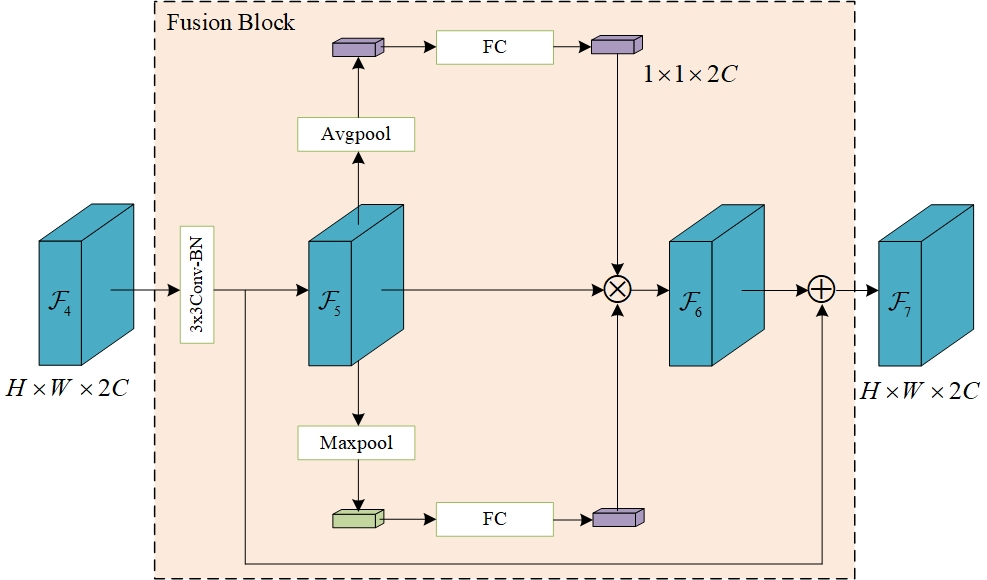
\includegraphics[width=0.7\columnwidth]{picture/LLIE/My Architecture/Fusion Block}
			%\captionsetup{font=scriptsize}
			\caption{
				\label{fig: Fusion Block} 
				融合模块的结构。
			}
		\end{figure}
		
		在 U-Net 网络编码器结构中,浅层特征包含丰富的纹理信息和颜色信息,多层卷积得到的高层特征包含全局信息。对于弱光图像增强,需要尽可能的保留输出结果中的颜色信息。为此,PACUT 结构引入了图像通道来保留具由特定颜色特征的信息,从而更好的恢复暗区信息,防止亮区信息过度曝光。具体来说,在 U-Net 网络中设计了三个条约链接,将浅层特征发送到后头,以解决颜色信息丢失的问题。为了有效的融合 ViT 和 U-Net 特征,提出一个如 Fig. \ref{fig: Fusion Block}所示的特征融合模块。其输入由两部分组成,即 PACUT 中 U-Net 分支得到的特征 $\mathcal{F_2}$ 和 ViT 分支中 Patch Expanding 后得到的特征 $\mathcal{F_3}$。该模块包含两个步骤。
		
		第一步,将两个尺寸为 $H \times W \times C$的特征图连接起来,形成一个尺寸为 $H \times W \times 2C$的特征图 $\mathcal{F}_4$。以该特征图为输入,通过 $3 \times 3$ 的卷积核,步长为1,进一步得到大小为 $H \times W \times 2C$ 的特征图 $\mathcal{F}_5$。这个过程可以有效的捕获颜色信息,表示为 
		
		\begin{equation}
			\begin{aligned}
				\mathcal{F}_5 = \delta \left( f^{3 \times 3} (\mathcal{F}_4)\right)
			\end{aligned}
			\label{eq: capture color information}
		\end{equation}
		
		在第二步中,通过为不同的通道分配适当的权重来重新校准特征映射 $\mathcal{F}_5$。为此,构建一个由两个加权支路和一个短连接组成的模块,如 Fig. \ref{fig: Fusion Block}所示。首先,通过全局平均池化将特征映射 $\mathcal{F}_5$ 压缩成 $1 \times 1 \times 2C$ 个向量;同时,特征映射 $\mathcal{F}_5$ 还需要进行全局最大池化,以尽可能的保留纹理细节。得到的 $1 \times 1 \times 2C$ 向量中的每一个元素表示通道信息。它们的公式为
		
		\begin{equation}
			\begin{aligned}
				\mathcal{Z}_{GAP} = \frac{1}{H \times W} \sum_{i}^{H} \sum_{j}^{W} {\mathcal{F}_5}_C (i,j)
			\end{aligned}
			\label{eq: avgpool}
		\end{equation}
		
		\begin{equation}
			\begin{aligned}
				\mathcal{Z}_{GMP} = \max \left( \mathcal{F}_5 \right)
			\end{aligned}
			\label{eq: maxpool}
		\end{equation}
		
		其中 $\mathcal{Z}_{GAP}$ 和 $\mathcal{Z}_{GMP}$ 分别为全局平均池化和全局最大池化得到的特征值,${\mathcal{F}_5}_C$ 为 $\mathcal{F}_5$ 的第 $C$ 个通道的特征。接下来,这两个压缩向量通过两个完全连接的层进行加权,以获得各自的权重向量。最后,通过特征向量乘以相应的权值,得到一个重新校准后,大小为 $H \times W \times 2C$ 的特征图 $\mathcal{F}_7$
		
		\begin{equation}
			\begin{aligned}
				\mathcal{F}_7 = \sigma \left( W_2 \delta (W_1 Z_{GAP}) \right) \cdot M \cdot \sigma \left( W_2 \delta (W_1 Z_{GMP})\right) +  \mathcal{F}_5
			\end{aligned}
			\label{eq: recalibrated feature map}
		\end{equation}
		
		其中 $W_1$ 和 $W_2$ 是两个完全连接层的权值。
		
		\subsection{Experimental Plan}

		实验的过程中,确保所有的实验在相同的硬件和软件环境下进行,并且为了确保结果的可靠性,可能需要多次运行实验并取平均值。我们主要基于 PyTorch 进行模型的搭建、训练和评估,使用 Matplotlib 库用于绘制图标和注意力图。基于 scikit-image 库计算 PSNR、SSIM 等评价指标。

		\subsubsection{Dataset}
		
		Tab. \ref{tab: Paired_training_datases} 展示了我们在实验中会使用到的弱光数据集,这些数据集包含真实数据与合成数据。对于每个数据集,我们需要进行如下操作:
		
		\begin{itemize}
			\item [$\bullet$]
			预处理: 确保所有图像都经过相同的预处理步骤,如尺寸调整、归一化等。
			
			\item [$\bullet$]
			分割: 将每个数据集分为训练集、验证集和测试集。
		\end{itemize}
		
		\subsubsection{Train}
		
		\begin{itemize}
			\item [$\bullet$]
			基线模型: 首先,训练基线模型(即完整的并行模型,包含完整的 CNN 和 Transformer 分支)。
			
			\item [$\bullet$]
			消融研究: 接着,训练去除 Transformer 分支的模型,以进行消融实验。
		\end{itemize}
		
		\begin{table}[!htbp]
			\centering
			\tiny
			%\resizebox{\textwidth}{!}{ %按照宽度调整调整表格大小
				\begin{tabular}{>{\centering\arraybackslash}m{2.5cm}|c|c|c|c}
					
					\hline
					
					\textbf{Name} & \textbf{Number} & \textbf{Format} & \textbf{Real/Syn} & \textbf{Video} \\
					
					\hline
					
					LOL\cite{wei2018deep} & 500 & RGB & Real & \\
					
					SCIE\cite{cai2018learning} & 4,413 & RGB & Real & \\
					
					VE-LOL-L\cite{jiang2019learning} & 2,500 & RGB & Real+Syn & \\
					
					MIT-Adobe FiveK\cite{bychkovsky2011learning} & 5,000 & Raw & Real & \\
					
					SID\cite{wei2018deep} & 5,094 & Raw & Real & \\
					
					DRV\cite{chen2019seeing} & 202 & Raw & Real & \checkmark  \\
					
					SMOID\cite{jiang2019learning} & 179 & Raw & Real & \checkmark  \\
					
					\hline
					
				\end{tabular}
				%}
			\captionsetup{font=scriptsize} %设置标题字体与表格字体一致
			\caption{\label{tab: Paired_training_datases}
				Summary of paired training datasets. 'Syn' represents Synthetic.} %表格的标题
			
		\end{table}
		
		\subsubsection{Performance Evaluation}
		
		对于每个数据集,使用以下指标评估模型性能:
		
		\begin{itemize}
			\item[$\bullet$]
			均方误差 (MSE)
			\item[$\bullet$]
			峰值信噪比 (PSNR)
			\item[$\bullet$]
			结构相似性指数 (SSIM)
			\item[$\bullet$]
			感知图像质量评估 (LPIPS)
		\end{itemize}
		
		\subsubsection{Contrast Experiment}
		
		\begin{itemize}
			\item[$\bullet$]
			跨数据集比较: 在所有数据集上评估基线模型的性能,并记录结果。
			\item[$\bullet$]
			消融实验: 在相同的数据集上评估去除 Transformer 分支的模型,并与基线模型进行比较。
		\end{itemize}
				
		\subsubsection{Attention Chart}
		
		\begin{itemize}
			\item[$\bullet$]
			CNN 分支: 可视化 CNN 分支的特征图,以展示模型如何处理局部特征。
			\item[$\bullet$]
			Transformer 分支: 可视化 Transformer 分支的注意力图,以展示模型如何处理全局特征。
		\end{itemize}
				
		\subsubsection{Results analysis and reporting}
		
		\begin{itemize}
			\item[$\bullet$]
			数据整理: 将所有实验结果整理成表格或图表。
			\item[$\bullet$]
			分析: 分析不同数据集和不同模型配置 (如有/无Transformer分支) 的性能差异。
		\end{itemize}
				
		\subsection{创新想法的调研支撑}
		
		\paragraph{Attention in CV}
		
		在计算机视觉领域,研究人员使用了不同类型的注意力机制,目的是使模型聚焦于图像本身。这大致分为两种类型:一种是基于通道的注意力机制,即 Squeeze-and-Excite。另一个是基于空间的注意力机制\cite{woo2018cbam}。然而,研究发现这些类型有三个局限性:
		
		\begin{itemize}
			\item[(1)] 
			卷积捕捉远距离特征的能力较差;
			
			\item[(2)]
			注意力机制关注所有输入;当分辨率较大时,计算成本增加;
			
			\item[(3)]
			不同时关注通道和空间维度关注信息。这就造成了信息的浪费和注意力的减弱。
		\end{itemize}	
		
		针对第一个限制 \cite{ramachandran2019stand} 将所有卷积替换为独立的自注意层和空间意识的独立自注意层,替换后的模型为纯注意模型。纯注意模型增强了网络对远距离特征连接的建模能力。在 ImageNet分类任务和 COCO 对象检测任务中,该模型优于使用卷积的基线模型。对于第三个限制,Woo 等人\cite{woo2018cbam}提出了一种卷积块注意模型 CBAM,这是一种轻量级的通用注意模型。该模型从通道维度和空间维度两方面关注重要信息。由于 CBAM 从多个维度提取重要信息,该模型被广泛应用于目标检测、目标分类等任务。实验表明,CBAM 模块可以显著提高网络的表达能力。同时,CBAM 可以搭配 SCConv\cite{li2023scconv}结构,SCConv 是一种名为可以即插即用的卷积模块,目的是减少卷积神经网络中特征之间的空间和通道冗余,从而压缩 CNN 模型并提高其性能。
		
		\paragraph{U-Net for LLIE}
		
		U-Net 网络由卷积层、下采样、上采样和跳过连接操作组成,其编码器和解码器具有对称结构。长期以来,U-Net 网络及其改进结构由于其强大的特征学习和特征重构能力,在图像语义分割领域取得了巨大的成功。U-Net 网络在弱光图像增强方面显示出出色的效果。Chen 等\cite{chen2018learning}创新性地提出了一种基于 U-Net 框架的弱光图像增强网络。该网络的核心架构是多尺度上下文聚合网络 (CAN) 和 U-Net 网络。之后的工作\cite{chen2018learning, zamir2021learning}也将 U-Net 架构应用到自己的网络中,其网络包含两个子网。即图像约简子网和感知损失子网,其中图像约简子网具有与\cite{chen2018learning}相同的 U-Net 架构。虽然\cite{chen2018learning, zamir2021learning}在使用U-Net架构增强图像方面取得了一定的效果,但\cite{meng2020gia}认为\cite{chen2018learning, zamir2021learning}网络忽略了全局信息,导致增强图像中的颜色不自然和物体伪影问题。为了改善以往网络的缺陷,利用 U-Net 架构,\cite{meng2020gia}在U-Net的编码器和解码器之间增加了全局信息感知模块(global information awareness module, GIA), GIA 可以将全局信息整合到整个网络中,改善增强图像中的颜色不一致和伪影。经过对\cite{chen2018learning, meng2020gia, zamir2021learning}的仔细研究,基于 U-Net 网络的弱光图像增强方法取得了很好的效果。然而,该网络仍然存在两个局限性:
		
		\begin{itemize}
			\item[(a)] 
			跳过连接只融合相同尺度的特征,导致编码器和解码器之间存在较大的语义差距;
			
			\item[(2)]
			全局上下文信息的连接相对稀缺。
		\end{itemize}	
		
		这两个限制容易导致增强图像的细节丢失、对比度差和颜色信息不准确。Zhou等\cite{zhou2018unet++,zhou2019unet++}改进了 U-Net 架构生成 U-Net++,在 U-Net++ 中将跳跃连接重新设计为一系列嵌套的密集跳跃连接,实现了多个特征的融合,加强了不同层次的特征信息接触。

		\paragraph{CNN for LLIE}
		
		CNN 在许多计算机视觉任务中表现出了令人印象深刻的结果。CNN 利用注意力机制\cite{yang2021locally, zhang2020attention}和上下文信息,从原始图像中生成注意感知并提取多尺度特征\cite{li2018multi,zamir2020learning}。基于 CNN 的低光图像增强方法不断发展。例如,基于 CNN 的自适应弱光图像增强框架\cite{li2020visual}极大地增强了图像对比度、颜色和细节信息。然而,现有的基于 CNN 的方法大多侧重于图像亮度、纹理和颜色的恢复\cite{xu2020learning}。由于局部光照不均匀,颜色信息和细节信息丢失严重,容易出现过增强或增强不足的问题。
		
%%%%%%%%%%%%%%%%%%%%%%%%%%%%%%%%%%%%%%%%%%%%%%%%%%%%%%%%%%%%%%%%%%%%%%%%%%%%%%%%%%%%%%%%%%%%%%%%%%%%
%%%%%%%%%%%%%%%%%%%%%%%%%%%%%%%%%%%%%%%%%%%%%%%%%%%%%%%%%%%%%%%%%%%%%%%%%%%%%%%%%%%%%%%%%%%%%%%%%%%%
%%                                                                                                %% 
%%								          Paper reading                                           %%
%%                                                                                                %%
%%%%%%%%%%%%%%%%%%%%%%%%%%%%%%%%%%%%%%%%%%%%%%%%%%%%%%%%%%%%%%%%%%%%%%%%%%%%%%%%%%%%%%%%%%%%%%%%%%%%
%%%%%%%%%%%%%%%%%%%%%%%%%%%%%%%%%%%%%%%%%%%%%%%%%%%%%%%%%%%%%%%%%%%%%%%%%%%%%%%%%%%%%%%%%%%%%%%%%%%%	

	
	\part{Paper Reading}
	
	\section{Lightweight Model}
		
		\subsection{(2023.8)1M parameters are enough? A lightweight CNN-based model for medical image segmentation}
		
		\paragraph{1M的参数就足够了吗?一种基于 CNN 的轻量级医学图像分割模型}
		
		\paragraph{(APSIPA ASC 2023 2区) doi: 10.1109/APSIPAASC58517.2023}
		
			\subsubsection{Research Background}
			
			卷积神经网络 (CNNs) 和基于 Transformer 的模型由于能够提取图像的 High-Level 特征和捕捉图像的重要方面而被广泛应用于医学图像分割。然而,在对高精度的需求和对低计算成本的期望之间往往存在权衡。具有更高参数的模型理论上可以获得更好的性能,但也会导致更高的计算复杂性和更高的内存使用率,因此实现起来并不实用。
			
			在本文中,作者寻找一种轻量级的基于 U-Net 的模型,它可以实现几乎相当甚至更好的性能,即 U-Lite。作者基于深度可分离卷积的原理设计了 U-Lite,这样该模型既可以利用神经网络的强度,又可以减少大量的计算参数。
			
			\subsubsection{Contribution}
			
			具体来说,作者提出了在编码器和解码器中都具有 $7\times7$ 的轴向深度卷积,以扩大模型的感受野。为了进一步提高性能,作者使用了几个具有 $3\times3$ 的轴向空洞深度卷积作为作者的分支之一。
			
			总体而言,U-Lite仅包含 878K 参数,比传统 U-Net 少35倍。与其他最先进的架构相比,所提出的模型降低了大量的计算复杂性,同时在医学分割任务上获得了令人印象深刻的性能。
			
			在本文中,作者重新思考了一种用于医学分割任务的高效轻量级架构,以进一步探索一种能够有效解决这一问题的高性能模型。
			
			简而言之,本文的主要贡献有3个方面:

			\begin{itemize}
				\item[(1)] 基于深度可分离卷积的概念,提出了轴向深度卷积模块的使用方法。该模块帮助模型解决每一个复杂的体系结构问题:扩大模型的感受野,同时减少沉重的计算负担。
				
				\item[(2)] 提出U-Lite,一种基于CNN的轻量级、简单的架构。据作者所知,U-Lite是为数不多的在性能和参数数量方面超过最近高效紧凑型网络UneXt的型号之一。
				
				\item[(3)] 作者已经在医学分割数据集上成功地实现了该模型,并取得了可观的效果。
			\end{itemize}
			
			\subsubsection{Approach}
			
			作者提出的 U-Lite 模型的概述如 Fig. \ref{fig: U-Lite Architecture} 所示。作者遵循 U-Net 的对称编码器-解码器架构,并以一种有效的方式设计U-Lite,以便该模型能够利用 CNN 的强度,同时保持计算参数的数量尽可能少。
			
			\begin{figure}[htbp]
				% read manual to see what [ht] means and for other possible options
				\centering 
				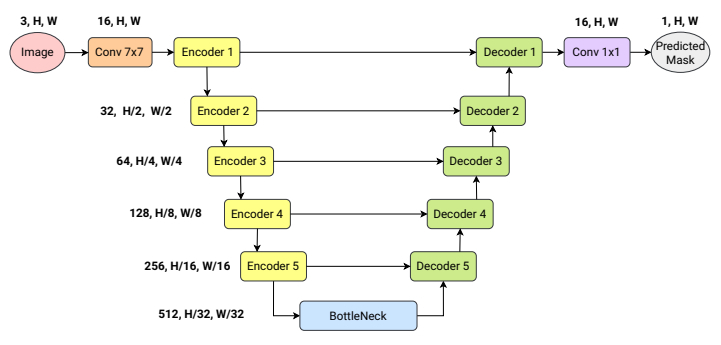
\includegraphics[width=\columnwidth]{picture/Lightweight Model/U-Lite Architecture}
				%\captionsetup{font=scriptsize}
				\caption{
					\label{fig: U-Lite Architecture} 
					The proposed U-Lite architecture.
				}
			\end{figure}
			
			为此,作者深思熟虑地提出了一个轴向深度卷积模块,如 Fig. \ref {fig: Axial Depthwise Convolution module} 所示。描述 U-Lite 的操作,形状为 $\left(3, H, W\right)$ 的输入图像通过 $3$ 个阶段被馈送到网络:编码器阶段、Bottleneck阶段和解码器阶段。U-Lite遵循分层结构,其中编码器提取形状$\left(C_i, \frac{H}{2^{i}}, \frac{W}{2^i}\right)$中的 $6$ 个不同 Level 的特征,其中 $i \in \{0,1,2, \ldots ,5\}$。
			
			\begin{figure}[htbp]
				% read manual to see what [ht] means and for other possible options
				\centering 
				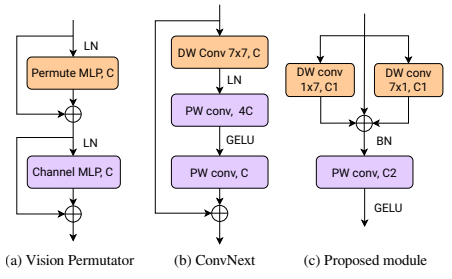
\includegraphics[width=0.6\columnwidth]{picture/Lightweight Model/Axial Depthwise Convolution module}
				%\captionsetup{font=scriptsize}
				\caption{
					\label{fig: Axial Depthwise Convolution module} 
					Architectures of (a) Vision Permutator, (b) ConvNext, and (c) Proposed Axial DW Convolution module. The proposed module is inspired by Vision Permutator’s and ConvNext's designs.
				}
			\end{figure}
			
			Bottleneck 和解码器参与处理这些特征,并将它们放大到原始形状以获得分割 Mask。作者还在编码器和解码器之间使用 skip connections 连接。值得注意力的是,尽管 U-Lite 的设计很简单,但由于轴向深度卷积模块的贡献,该模型在分割任务上仍然表现良好。
			
			\paragraph{Axial Depthwise Convolution module}
			
			视觉 Transformer 的成功推动了研究和改进这种特殊结构的各种工作。Swin-Transformer 通过将自注意力计算限制在大小为 $7 \times 7$ 的非重叠局部窗口,降低了 Transformer 的计算复杂性。ConvNext 实现了这一修改,并在 CNN 架构中采用了 kernel 大小为 $7 \times 7$ 的卷积,使 ResNet 在 ImageNet 上的最高精度达到 $86.4\%$。
			
			Vision Permutator 利用线性投影来沿着高度和宽度维度分别编码特征表示。
			
			\textbf{论文提及:如果用局部感受野\footnote{局部感受野(Local Receptive Field)指的是一个神经元只对输入数据的一个局部区域进行响应,这有助于捕捉图像中的局部特征,如边缘、角点等。}取代ViT的十字形感受野\footnote{十字形感受野(Cross-shaped Receptive Field)指的是在ViT中,每个注意力头计算的是全局的自注意力,这意味着每个输出位置的注意力是基于整个输入图像的。但在一些变体中,例如CrossViT,会使用十字形的感受野,即在水平和垂直方向上分别计算注意力,以减少计算量并捕捉不同方向的特征。},就像 Swin Transformer\footnote{Swin Transformer 利用局部感受野取代十字感受野,它将输入图像划分为多个小块,然后在这些小块内部计算自注意力,从而实现局部感受野。其可以减少计算量,增强模型的泛化能力,并提高效率。} 对 ViT 所作的那样,会发生什么?}
			
			因此,作者提出了轴向深度卷积模块,作为Vision Permutator和卷积设计的组合。该算子的数学公式表示为
			
			\begin{equation}
				\begin{aligned}
					x^\prime = x + \text{DW}_{1 \times n}(x) + \text{DW}_{n \time 1}(x) \\
					y = \text{GELU}\left(PW_{C_1 \rightarrow C_2} \left(\text{BN}\left(x^\prime \right)\right)\right)
				\end{aligned}
				\label{eq: Axial Depthwise Convolution module}
			\end{equation}
			
			\begin{figure}[htbp]
				% read manual to see what [ht] means and for other possible options
				\centering 
				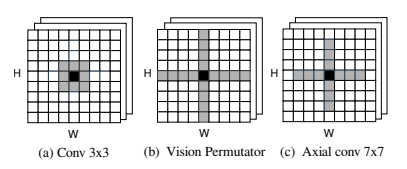
\includegraphics[width=0.6\columnwidth]{picture/Lightweight Model/Receptive Field}
				%\captionsetup{font=scriptsize}
				\caption{
					\label{fig: Receptive Field} 
					The receptive field comparison between Convolution $3 \times 3$,
					Vision Permutator, and Axial convolution $7 \times 7$. Axial convolution
					$7 \times 7$ offers a large receptive field compared with Convolution
					$3 \times 3$ while using fewer computational parameters than Vision
					Permutator.
				}
			\end{figure}
			
			其中,$x$为输入特征,$y$为输出特征;DW、PW和BN分别代表深度卷积、点卷积和批量归一化,$1 \times n$和$n \times 1$是卷积的 kernel 大小;$C_1$ 和 $C_2$ 表示特征图的输入和输出通道的数量。在作者的实验中,$n=7$。为了实现最小和灵活的设计,作者使用了一种独特的逐点卷积,而不添加残差连接,允许自适应地改变输入通道的数量。
			
			\paragraph{Encoder Block and Decoder Block}
			
			编码器和解码器块的设计原理如下:
			
			\begin{itemize}
				\item [(1)] 遵循深度可分离卷积架构。这是从头开始成功构建轻量级模型的重要关键。深度可分离卷积在使用较少参数的同时,提供了与传统卷积相同的性能,从而降低了计算复杂性,使模型更加紧凑。
				\item [(2)] 限制使用不必要的操作op。只需使用普通的MaxPooling和UpSampling层。不需要诸如转置卷积之类的高参数消耗算子。逐点卷积算子可以同时扮演两个角色:沿着特征图的深度对特征进行编码,同时灵活地改变输入通道的数量。
				\item [(3)] 每个编码器或解码器块采用一个批量标准化层,并以GELU激活功能结束。作者对批处理规范化和层规范化进行了性能比较,但没有太大区别。应用GELU是因为与ReLU和ELU相比,在使用GELU时证明了其在准确性方面的改进。
			\end{itemize}
			
			U-Lite的编码器和解码器结构如 Fig. \ref{fig: Encoder and Decoder} 所示。
			
			\begin{figure}[htbp]
				% read manual to see what [ht] means and for other possible options
				\centering 
				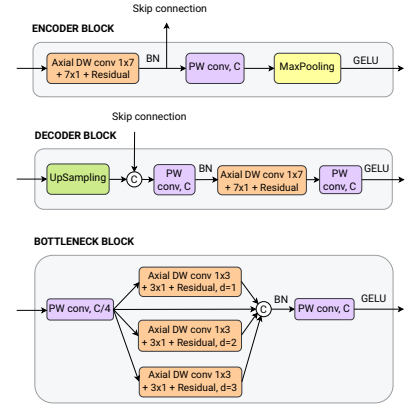
\includegraphics[width=0.6\columnwidth]{picture/Lightweight Model/Encoder and Decoder}
				%\captionsetup{font=scriptsize}
				\caption{
					\label{fig: Encoder and Decoder} 
					Encoder, decoder, and bottleneck blocks. Designed based on Depthwise Separable Convolution concept. Each block adopts one Batch Normalization layer and ends with a GELU activation function.
				}
			\end{figure}
			
			\paragraph{Bottleneck Block}
			
			为了进一步提高U-Lite的性能,作者将kernel大小 $n=3$ 的轴向扩展深度卷积应用于 Bottleneck 块。应用的空洞率为 $d = 1,2,3$。作者使用具有大小为3的 kernel 的轴向扩张卷积,原因有两个:
			
			\begin{itemize}
				\item [(1)] 大小为3大小的kernel更适合底层特征的空间形状,其中这些特征的高度和宽度减少了多次。
				
				\item [(2)] 当使用具有不同空洞率的空洞卷积来捕获后面阶段的High-Level特征的多空间表示时,它给出了更好的性能。
			\end{itemize}
			
			为了进一步减少可学习参数的数量,在 Bottleneck 块的开头采用了逐点卷积层。这有助于在将最后一层特征提供给轴向扩展深度卷积机制之前缩小其通道尺寸。
			
			\subsubsection{Future}
		
			-
	\section{Edge Detection}
		
		\subsection{(2022.3)Survey of Image Edge Detection}
			
		\paragraph{图像边缘检测综述}
			
		\paragraph{(Frontiers in Signal Processing 2区) doi: 10.3389/frsip.2022.826967}
			
			\subsubsection{Research Background}
				
			作者对边缘检测算法进行全面的分析和专题研究。首先,通过对传统边缘检测算法的多层次结构进行分类,介绍了各类算法的原理和方法。其次,重点分析了重点分析了基于深度学习的边缘检测算法,分析了各算法的技术难点、方法优势以及骨干网络选择。然后,通过在BSDS500和NYUD数据集上的实验,进一步评估了每种算法的性能。可以看出,目前的边缘检测算法的性能已经接近甚至超越了人类视觉水平。目前,关于图像边缘检测的综合综述文章较少。本文致力于对边缘检测技术进行全面的分析,旨在为相关人员轻松跟进边缘检测的最新发展并做出进一步的改进和创新提供参考和指导。
			
			\subsubsection{Contribution}
			
			由于图像边缘的重要性,图像边缘检测自提出以来就受到了研究人员的广泛关注,Fig. \ref{fig: Development} 说明了边缘检测算法的发展。
			
			\begin{figure}[htbp]
				% read manual to see what [ht] means and for other possible options
				\centering 
				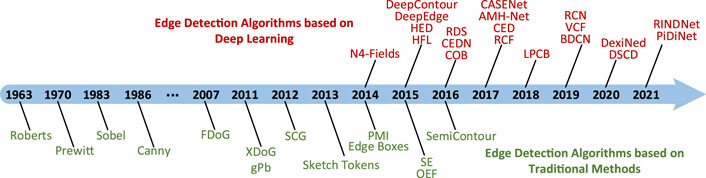
\includegraphics[width=\columnwidth]{picture/Edge Detection/Development}
				%\captionsetup{font=scriptsize}
				\caption{
					\label{fig: Development} 
					Development of edge detection algorithms based on traditional and deep learning methods.
				}
			\end{figure}
			
			随着深度学习的不断发展,出现了各种基于 CNN 实现边缘检测的方法。2015 年,Bertasius 等人。改变了传统的自下而上的边缘检测思路,提出了一种自上而下的多尺度发散深度网络 DeepEdge \cite{bertasius2015high} 用于边缘检测。同年,Xie等人开发了整体嵌套边缘检测算法HED\cite{xie2015holistically},解决了基于图像的整体训练和预测以及多尺度多层次特征学习的问题。 2017年,Liu等人,提出了一种使用更丰富的卷积特征的精确边缘检测器RCF\cite{liu2017richer}。 2019年,Deng等人,提出了一种新颖的端到端边缘检测系统DSCD\cite{deng2020deep},它有效地利用多尺度和多层次特征来产生高质量的物体边缘输出。 2021年Su等人,设计了 PiDiNet\cite{su2021pixel},一种简单、轻量级且高效的边缘检测架构。
			
			\subsubsection{Approach}
			
			\paragraph{Evaluation Indicators}
			
			最佳数据集尺度 (Optimal Dataset Scale, ODS) 和最佳图像尺度 (Optimal Image Scale, OIS) 是评估图像轮廓生成结果时使用最广泛、最具代表性的评价指标,此外还有常用的每秒帧数 (Frames Per Second, FPS) 和精确召回率 (Precision-Recall, PR) 曲线。ODS-F和OIS-F中的F值是Precision(P)和Recall(R)的总和平均值,并被表示为Eq. \ref{eq: F-Score}。
			
			\begin{equation}
				\begin{aligned}
					\text{F-Score} = \left(1+\beta^2\right) \cdot \frac{Precision \cdot Recall}{\beta^2 \cdot Precision + Recall}
				\end{aligned}
				\label{eq: F-Score}
			\end{equation}
			
			通过调整$\beta$的值,准确度和召回率的显著性程度是可以控制的,如果$\beta = 1$,表示为Eq. \ref{eq: F-Score1};如果$\beta = 0$,表示为Eq. \ref{eq: F-Score2};如果$\beta = \infty$,表示为Eq. \ref{eq: F-Score3}。
			
			\begin{equation}
				\begin{aligned}
					\text{F-Score} = \frac{2Precision \cdot Recall}{Precision + Recall}
				\end{aligned}
				\label{eq: F-Score1}
			\end{equation}
			
			\begin{equation}
				\begin{aligned}
					\text{F-Score} = Precision
				\end{aligned}
				\label{eq: F-Score2}
			\end{equation}
			
			\begin{equation}
				\begin{aligned}
					\text{F-Score} = Recall
				\end{aligned}
				\label{eq: F-Score3}
			\end{equation}
			
			最佳数据集尺度 (Optimal Dataset Scale, ODS) 对数据集内所有的图像设置相同的阈值,即固定阈值$\beta$选择并应用于所有图像,以便最大化整个数据集上的 F 分数。
			
			最佳图像尺度 (Optimal Image Scale, OIS) 对每幅图像上设置不同的阈值$\beta$选择最大化该图像的F分数。
			
			每秒帧数 (Frames Per Second, FPS),即目标网络每秒可以检测到多少张图像以及图像刷新的频率。用于评价目标检测的速度,时间越短,检测速度越快。
			
			精确召回率 (Precision-Recall, PR) 曲线,PR曲线是用精度和召回率两个变量绘制的曲线,其中精度为纵坐标,召回率为横坐标,广泛应用于信息提取领域,表示正样本中实际为正的比例。
			
			\paragraph{Backbone Network}
			
			主干网络是边缘检测任务的基本特征提取器,强大的主干网络可以提取更丰富的图像特征。目前大多数基于深度学习的边缘检测模型都使用 AlexNet\cite{krizhevsky2012imagenet}、VGG16\cite{simonyan2014very} 和 ResNet\cite{he2016deep} 作为骨干网络。
			
			Alex等人在2012年的ImageNet竞赛中提出了AlexNet网络。该网络赢得了当年的ImageNet LSVRC,准确率远高于第二名,成为深度学习的又一亮点。AlexNet网络包含8个学习层——5个卷积层和3个全连接层,含有6000万个参数和65万个神经元。引入了Relu激活函数、数据增强、Dropout和级联池化操作,以防止过拟合并提高模型的整体泛化能力。作者发现,模型的深度似乎在神经网络的性能中起着重要作用,这一发现也启发了后来VGG和ResNet网络的结构设计。基于网络重构的边缘检测算法AMH-Net和N4-Fields网络随后使用AlexNet网络作为基础网络。
			
			Simonyan和Zisserman 在2014年设计了深度卷积网络VGG16,由13个卷积层和3个全连接层组成,旨在研究大规模图像识别中卷积网络深度的准确性。Simonyan等人发现,使用非常小的3×3卷积滤波器将神经网络深度推进到16-19个权重层,可以显著提高VGG模型的性能。它采用了更深的网络结构,结合较小的卷积核和池化核,使其在有效控制模型参数大小的同时获得更多的图像特征,避免了大量计算和复杂结构,同时实现了先进的性能。此外,VGG模型具有良好的泛化能力,可以很好地推广到其他图像处理领域。因此,该模型现在是基于深度学习的图像边缘检测算法中最受欢迎的骨干网络。
			
			ResNet (2016年):尽管网络的深度对模型的性能至关重要,但实验上认为深度网络提取更复杂的特征结构。实验发现,随着网络深度的增加,梯度消失或爆炸,导致网络准确率饱和甚至下降。何等人(2016年)设计了深度残差网络 (Deep Residual Network)。作者识别了深度模型的“退化”问题,并提出了“快捷连接”的解决方案。ResNet通过引入残差学习,极大地消除了由于过度深度导致的神经网络训练困难问题,使得网络深度首次超过100层,甚至可以超过1000层。边缘检测模型COB和AMH-Net的设计基于ResNet的一些思想。
			
			\subsubsection{Future}
			
			-
			
			

		
		\renewcommand{\refname}{References}
		
		
		%	\begin{thebibliography}{00}
			
			%		\bibitem{b1}\label{cite:b1}
			%		W. Wang, C. Wei, W. Yang and J. Liu, "GLADNet: Low-Light Enhancement Network with Global Awareness," 2018 13th IEEE International Conference on Automatic Face \& Gesture Recognition (FG 2018), Xi'an, China, 2018, pp. 751-755, DOI: 10.1109/FG.2018.00118.
			
			%		\bibitem{b2}\label{cite:b2}
			%		A.\ Mahajan, K.\ Somaraj and M. Sameer, "Adopting Artificial Intelligence Powered ConvNet To Detect Epileptic Seizures," 2020 IEEE-EMBS Conference on Biomedical Engineering and Sciences (IECBES), Langkawi Island, Malaysia, 2021, pp. 427-432, DOI: 10.1109/IECBES48179.2021.9398832.
			
			%		\bibitem{Cyr}
			%		N.\ Cyr, M.\ T$\hat{e}$tu, and M.\ Breton,
			% "All-optical microwave frequency standard: a proposal,"
			%		IEEE Trans.\ Instrum.\ Meas.\ \textbf{42}, 640 (1993).
			
			
			
			%	\end{thebibliography}
		
		\bibliographystyle{unsrt}
		\bibliography{reference}
		
		
	\end{document}
